% !TEX root = ../my-thesis.tex
%

\chapter{Benchmark}
\label{sec:Benchmark}

\cleanchapterquote{Un petit chapitre pour le doctorant, un grand chapitre pour l'humanité}{Doctorant anonyme}{(Citation temporaire)}

\section{Propriétés}
\label{sec:Benchmark}

Dans ce chapitre, nous abordons la conception d'un banc de test permettant l'étude quantitative des filtres de rehaussement. Notre banc de test permet d'appliquer plusieurs instances de paramètres d'un filtre sur une base de données. Le résultat du filtrage est ensuite seuillé et les métriques d'évaluations sont calculées dans des zones d'intérêts définies par l'utilisateur. Une fois les métriques collectées, celles-ci peuvent être exploitées indépendamment par des outils de traitement de données. 

La création de notre banc de test passe par la construction d'une interface de filtres unifiés, la construction des jeux de données, la création de zones d'évaluations et le choix des métriques d'évaluations. Cette construction s'est faite de manière itérative au fur et à mesure des observations faites durant les expériences dont les résultats sont présentés dans le chapitre suivant.

\tikzstyle{capNode} = [rectangle, rounded corners, minimum width=3cm, minimum height=1cm,text centered, draw=black]
\tikzstyle{capNodeRed} = [rectangle, rounded corners, minimum width=3cm, minimum height=1cm,text centered, draw=red]
\tikzstyle{cNode} = [circle, minimum width=1cm, minimum height=1cm, text centered, draw=black, fill=white!30]
\tikzstyle{arrow} = [thick,->,>=stealth]

\begin{figure}[t!]
  \centering
  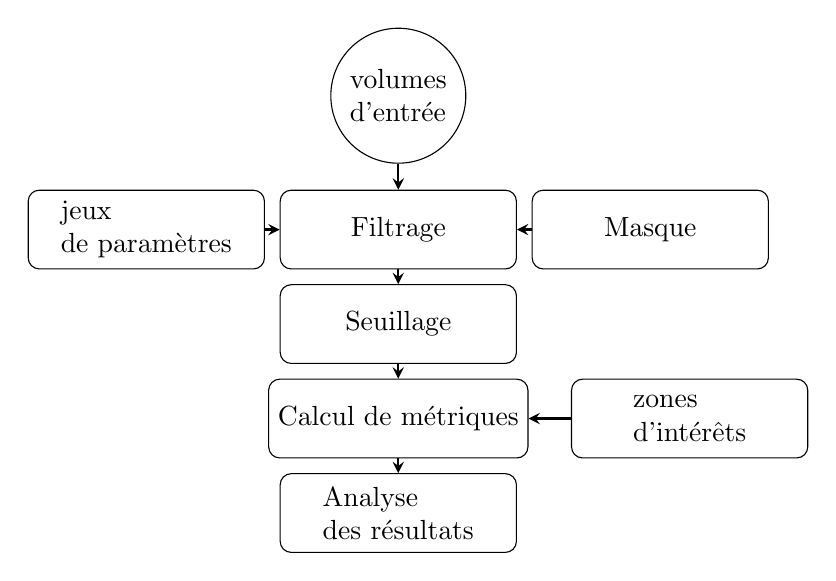
\begin{tikzpicture}[node distance=1.2cm]
    \node (input)[cNode,align=left] {volumes \\ d'entrée};
    \node (filtrage)[capNode, below of=input,align=left,yshift=-0.5cm] {Filtrage};
    \node (parametres)[capNode, left of=filtrage,align=left,xshift=-2cm] {jeux \\ de paramètres};
    \node (Masques)[capNode, right of=filtrage,align=left,xshift=2cm] {Masque};
    \node (seuillage)[capNode, below of=filtrage, align=left] {Seuillage};
    \node (metriques)[capNode, below of=seuillage, align=left] {Calcul de métriques};
    \node (ZI)[capNode, right of=metriques, align=left,xshift=2.5cm] {zones \\ d'intérêts};
    \node (traitement)[capNode, below of=metriques, align=left] {Analyse \\ des résultats};
  
    \draw [arrow] (input) -- (filtrage);
    \draw [arrow] (filtrage) -- (seuillage);
    \draw [arrow] (parametres) -- (filtrage);
    \draw [arrow] (Masques) -- (filtrage);
    \draw [arrow] (ZI) -- (metriques);
    \draw [arrow] (seuillage) -- (metriques);
    \draw [arrow] (metriques) -- (traitement);

  \end{tikzpicture}
  \caption{Schéma global du banc de test}
\end{figure}

Se baser sur la littérature pour choisir un filtre de rehaussement pour une application spécifique n'est pas une tâche simple. La littérature permet de se faire une vision globale sur ces filtres et présente de nombreux exemples d'applications. Cependant, leur incorporation dans une chaine de traitements dilue l'évaluation de leur impact réel sur la segmentation. Elle rend aussi plus difficile le choix d'un filtre et ses paramètres optimaux pour une modalité et un organe spécifique. De plus les métriques de références varient aussi entre deux publications ajoutant à la difficulté d'établir une comparaison. Il est donc nécessaire de proposer une base de comparaison unifiée.

% redite culinaire, pour fixer l'idée
%Si on utilise une métaphore, cela revient à évaluer le meilleur chocolat à partir de trois expériences : La première compare du chocolat blanc et du chocolat noir au goût ; la seconde du chocolat noir fourré à la praline et du chocolat au lait à l'odeur ; la troisième du chocolat au lait et pépites de caramel avec du chocolat noir aux fruits rouges à leur texture. Hiérarchiser les avantages de chaque chocolats devient alors complexe.

 Quelques travaux proposent une comparaison entre filtres de rehaussement. Par exemple Obara, Sazak et Alharbi \cite{Sazak2019_bowler_hat_2D} \cite{Alharbi2018_TP_2D_3D} ont proposé une comparaison de filtres 2D et 3D à base d'hessiennes et de tenseurs de phase, ces articles donnent toutefois une part très importante à l'évaluation qualitative plutôt que quantitative. De plus, ils ne proposent pas de discussion sur l'impact de la paramétrisation des filtres. En 3D, une analyse quantitative des filtres de rehaussement sur un grand nombre de volumes a été réalisé par Manh Luu en 2015 \cite{Luu2015_liver_vesselness_comparison} et Phellan \cite{Phellan2017_Brain_vesselness_comparison} en 2017.

Manh Luu a proposé un banc de test sur 51 images tomodensitométriques du foie sans prétraitement des données. Il ajoute cependant une segmentation à base de croissance de région dans sa chaine de traitement. Dans ce travail, l'évaluation de la qualité de la segmentation est basée sur des échantillons de points positionnés à l'intérieur et autour des vaisseaux. Les filtres testés sont Frangi,Sato, Erdt et les schémas de diffusion HDCS, VED et RPM. Les paramètres des filtres sont optimisés sur une sous section de la base de donnée. L'optimisation des paramètres est un fait suffisamment rare dans la littérature pour être souligné. Les métriques utilisées pour l'évaluation des filtres sont le ratio contraste-bruit (SNR), le rappel, la précision (accuracy) et la spécificité.

Phellan quant à lui propose un banc de test sur 5 images IRM du cerveau et 40 volumes générés avec    VascuSynth et l'ajout d'artefacts de tomodensitométrie. Sa chaine de traitement inclus un prétraitement des données et une segmentation à base de seuillages et d'un filtrage de composantes connexes. Sa méthode d'analyse repose sur des vérités terrains binaires du réseau vasculaire entier et sur l'évaluation du diamètre des vaisseaux. Les filtres évalués par Phellan sont Frangi, Sato, Erdt, OOF, RORPO, WTH et les schémas de diffusion HDCS, VED et RPM. Seul les paramètres d'échelles sont optimisés dans ces travaux, les paramètres intrinsèques par défaut étant fixé par l'auteur. Les performances des filtres sont évaluées grâce au Dice au MCC à l'analyse de courbes ROCS et une analyse en composantes connexes.

Ces deux bancs de test proposent des méthodes d'évaluations différentes. Pour notre application, des points positifs sont présents dans les deux benchmarks, qui chacun recouvre une partie de nos besoins sans toutefois y répondre complètement... En effet, l'évaluation de Manh Luu sur le foie n'est pas faite sur une segmentation voxélique. Celle de Phellan est réalisée sur un autre organe sans optimisation des paramètres. Des filtres récents ne sont pas évalués, car ils sont postérieurs aux publications. Nous voulions aussi évaluer les filtres sur des zones spécifiques définis tels que les bifurcations des vaisseaux. C'est pourquoi nous avons voulu créer notre propre banc de test, avec pour objectif l'imagerie du foie. Nous avons voulu éviter de tomber dans le piège des travaux précédents en proposant une base suffisamment global pour s'accommoder de différentes modalités et suffisamment modulaire pour être utilisé pour des expériences diverses, et être prises en main par d'autres utilisateurs.

\section{Homogénéisation des filtres}
\label{sec:Filtres}

Former une base homogène de filtres n'est pas une tâche simple. Celle-ci nécessite la recherche de code existant ou d'implémenter les filtres en se basant sur la méthodologie de l'article original.

Réaliser l'implémentation d'un filtre à partir des indications de l'auteur est parfois complexe, car il doit souvent se soumettre à un exercice de concision lors de la publication de ses travaux. L'auteur va donc à l'essentiel et certains détails d'implémentation peuvent être omis. La difficulté peut aussi survenir d'un problème de compréhension de la part du lecteur, surtout lorsque les articles sont écrits dans une langue étrangère à la sienne. Il faut donc être particulièrement attentif à la compréhension et à la vérification des hypothèses afin d'implémenter correctement les filtres. 

La collecte d'implémentations existantes n'est pas non plus évidente. En effet, il est possible que plusieurs versions d'un algorithme existent. Il est alors nécessaire de vérifier le code en détail. Certaines implémentations peuvent présenter des interfaces différentes de l'article original et nécessiter un travail de translation d'une interface à l'autre. Il arrive aussi que des codes soient disponibles, mais avec une dette technologique importante suite à l'évolution des logiciels ou des librairies nécessaires à leur fonctionnement. Enfin, la multiplicité des langages, des librairies et des logiciels sur lesquels sont déployés les filtres ajoute au temps dédié à cette tâche. Ce travail est souvent réalisé de manière isolée par un chercheur, un doctorant, ou stagiaire pour leurs expériences personnelles et ne profite pas à la communauté personne travaillant sur le sujet. Elle doit alors reprendre d'elle-même la totalité de ce travail à chaque introduction d'une nouvelle méthode.

Dans nos travaux, nous avons sélectionné, adapté et implémenté sept filtres qui répondent tous à une problématique spécifique du rehaussement TABLE~\ref{Tab:available_vesselness}. La diversité de leur origine est résumée dans la table TABLE~ \ref{Tab:origins_vesselness}. Il a été choisi d'implémenter ces filtres et leurs modifications en C++ avec la librairie ITK. Le C++ est particulièrement connu pour sa rapidité, un élément crucial pour des applications 3D qui doivent traiter un nombre important de voxels. La librairie open source ITK (insight toolkit), développée par Kitware Inc. depuis 2001, est la plus grosse librairie de traitement d'images médicales. Elle fournit un ensemble de briques algorithmiques déjà implémentées et a l'avantage de lire nativement une grande diversité de formats d'images médicales ce qui est un atout la diffusion de notre banc de test.

Cette librairie a une communauté active et connait des mises à jour régulières. C'est à la fois un avantage, pour la correction de bugs et l'introduction de nouveaux algorithmes et un inconvénient, car la dette technologique s'accumule plus rapidement à causes de cycles plus courts entre deux versions.


\begin{table}
    \begin{center}
  \begin{tabular}{l|l|l}
  Méthode   &  Idée centrale                                                                       & Date \\ \hline  \hline 
  Sato      & Reconnexion des vaisseaux, contrôle du bruit                                         & 1997 \\ \hline
  Frangi    & Contrôle sur l'atténuation des structures en plateau et en blobs                     & 1998 \\ \hline
  Meijering & Détections de fines structures allongées                                             & 2004 \\ \hline
  OOF       & Limitation du débordement des réponses lié à l'espace d'échelle gaussien             & 2010 \\ \hline
  Jerman    & Contrôle de l'homogénéité des réponses des vaisseaux                                 & 2016 \\ \hline
  Zhang     & Pré-traitement pour limiter le rehaussement des bordures du foie (TDM foie)          & 2018 \\ \hline
  RORPO     & Détection par chemins et différentiation des vaisseaux par vote sur les orientations & 2018  
  \end{tabular}
  \end{center}
  \caption{Méthodes disponibles et idées principales guidant leurs conceptions}
  \label{Tab:available_vesselness}

  \end{table}

  \begin{table}
    \begin{center}
        \begin{tabular}{l|l|l|l}
            Méthode   &  Provenance                                     & État \\ \hline  \hline 
            Sato      & librairie ITK (C++)                             & prêt à l'emploi \\ \hline
            Frangi    & librairie ITK (C++)                             & prêt à l'emploi \\ \hline
            Meijering & Github (Matlab), scipy                          & pondération proposée étrange  \\ \hline
            OOF       & Site de l'auteur (Matlab), insight journal (C++)& obsolète \\ \hline
            Jerman    & Github de l'auteur (Matlab)                     & prêt à l'emploi \\ \hline
            Zhang     & Non disponible                                  & non implémenté \\ \hline
            RORPO     & Github de l'auteur (C++)                        & prêt à l'emploi  
        \end{tabular}
    \end{center}
    \caption{Origine des méthodes}
    \label{Tab:origins_vesselness}
  \end{table}

La conception de notre banc de test a été guidé par plusieurs axes majeurs.
  
Le premier axe de conception a été d'évaluer le rehaussement pour la segmentation de voxélique. L'analyse à partir d'un ensemble de marqueurs comme réalisé par Manh Luu nous a paru trop imprécise pour rendre de compte de la totalité du profil du rehaussement. Nous avons aussi voulu éviter au maximum des traitements supplémentaire avant et après le rehaussement afin d'évaluer au plus près les filtres. La segmentation voxélique s'imposait donc comme le meilleur choix. La natu
re des vérités terrains des jeux de données disponibles et une plus grande quantité d'applications annexes (maillages, simulation de flux) pouvant servir au projet R-Vessel-X  nous a conforté dans ce choix.

\subsection{Redéfinition du domaine de sortie des filtres}
Le rehaussement de vaisseaux est parfois présenté comme une carte chaleur ou de probabilité pour lesquels une quantité d'appartenance à un vaisseau est associé à chaque voxels. Pour le filtre de Frangi cette quantité est définie entre 0 et 1. Cette propriété est désirable dans de nombreuses applications, car elle est plus simple à intégrer dans des chaînes de traitement que des filtres définis sur des domaines plus larges. Elle est aussi plus simple à interpréter.

Cependant, la réponse de tous les filtres ne partage pas nécessairement cette propriété. Par design seuls Jerman et Zhang ont une réponse définie sur cet intervalle. La réponse de Sato est définie sur $[0,+\infty]$, tout comme celle d'OOF et de Meijering. RORPO est un cas particulier, car l'intensité de sortie du filtre dépend de l'intensité maximum de l'image source. En effet, RORPO se base sur des ouvertures morphologiques dont la définition est bornée par le domaine de l'image. 

Dans une optique de généralisation et de diffusion des filtres, nous partons du principe que les images des bases de données ne sont pas normalisées. On ne peut donc pas espérer une stabilité des filtres à partir de leur entrée. Il faut donc contraindre les sorties des filtres entre zéro et un. Nous avons choisi pour Sato, OOF et Meijering de normaliser la réponse de sortie en fonction de la plus grande valeur de sortie du filtre $ \frac{I_{rehaussement}(x)} {max(I{rehaussement}(x))} $. Pour RORPO dont la sortie est liée à l'intensité de l'image d'entrée la normalisation prend la forme $ \frac{I_{rehaussement}(x)} {max(I(x))} $.
La nature de RORPO en fait un filtre difficile à intégrer à notre banc de test. En effet, l'utilisation de la morphologie implique une utilisation ``tout ou rien'', à mi-chemin entre segmentation binaire et rehaussement. On conserve en effet seulement les intensités des voxels candidats à la participation de structures tubulaires sans leur associer de degrés d'appartenances. Cette segmentation en niveau de gris force l'utilisation d'une normalisation non naturelle afin de passer à une carte de probabilité nécessaire pour l'évaluation de ce benchmark. Cette procédure a un impact non négligeable sur le résultat des expériences présentées dans le chapitre suivant.

Une attention particulière doit être portée aux types d'images pris en charge par l'implémentation des filtres. En effet, la dynamique des images médicales n'est pas commune. Une image 2D classique est souvent représentée sur 8 bits exprimant 256 niveaux de gris $[0,255]$ (multiplié par 3 canaux pour les images couleurs). Les images médicales possèdent la plupart du temps un seul canal avec parfois une dynamique de niveaux de gris plus importante de 16 ou 32 bits et peuvent présenter des valeurs négatives. Il faut donc s'assurer que les filtres supportent les images. Par exemple, l'implémentation de RORPO ne supporte que des valeurs de pixels positifs et nécessite de faire une translation des niveaux de gris négatifs sous peine d'obtenir des comportements non définis.

\subsection{Utilisation de masques}

Il peut souvent être utile de ne traiter qu'une partie de l'image, par exemple lorsqu'un ne veut rehausser les vaisseaux que d'un organe en particulier. La manière la plus simple est de définir un masque binaire de la même taille que l'image. On renseigne pour chaque voxel s'il appartient à la zone à traiter (1 ou 255) ou s'il n'y appartient pas(0). Là encore, il faut être attentif à l'implémentation du masque. Une première implémentation consiste appliquer le masque sur le rehaussement après coup. Le filtre est appliqué à toute l'image avant de ne conserver que la partie concernant l'organe observé. Cette implémentation a le désavantage de calculer le rehaussement dans des zones non utilisées par la suite. Une seconde implémentation consiste à masquer l'image dans un premier temps, puis de calculer le rehaussement dans cette image masquée. On gagne ainsi du temps de calcul dans les zones nulles. Ce gain de temps n'est pas négligeable, puisqu'un banc de test applique de multiples fois les filtres sur un grand nombre de volumes 3D. Cependant, masquer en aval du rehaussement créé artificiellement de faux rebords avec un différentiel d'intensités marqué.
 
\begin{figure}
  \centering
  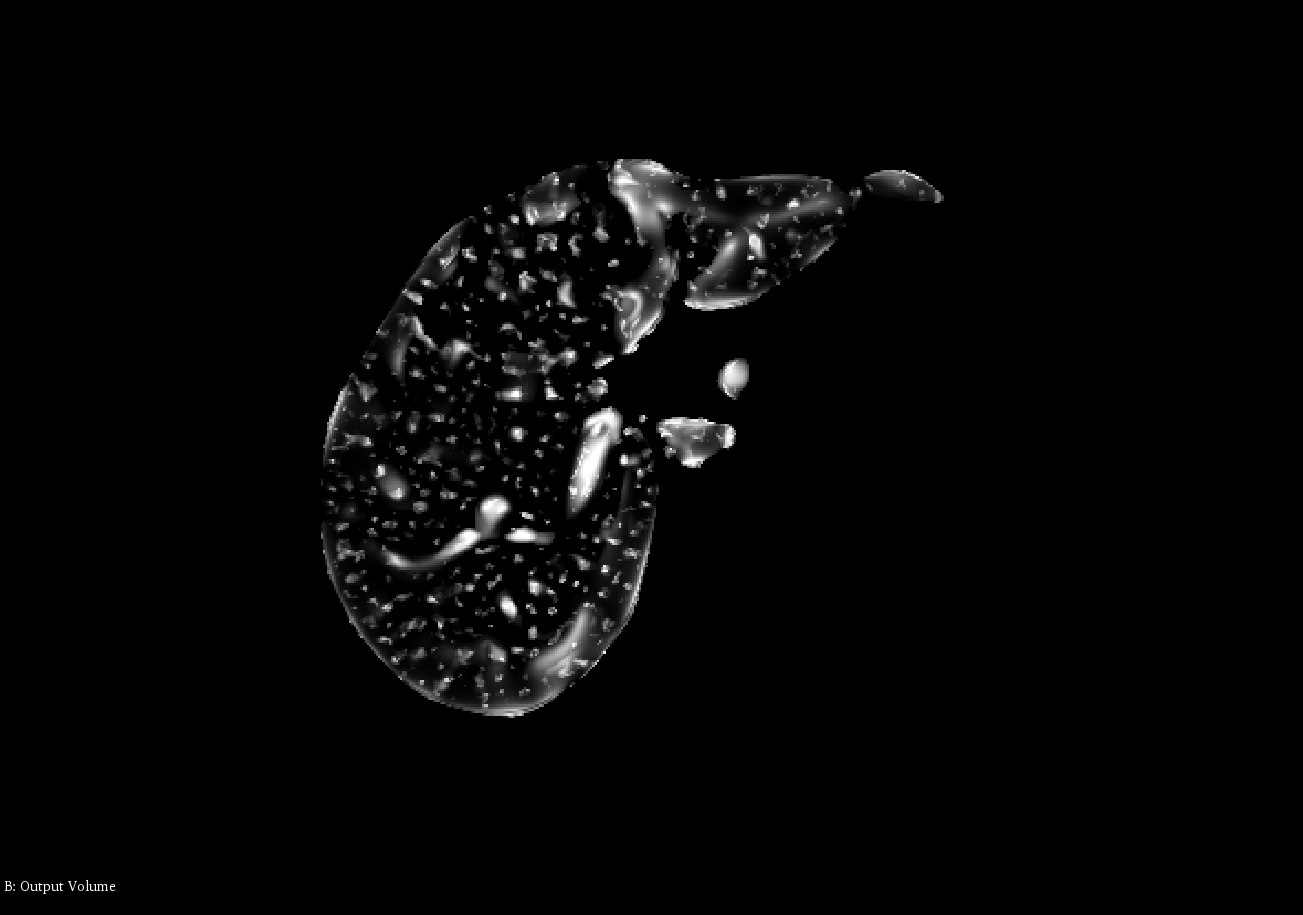
\includegraphics[height=3cm]{Images/output_maskedFirst.png}
  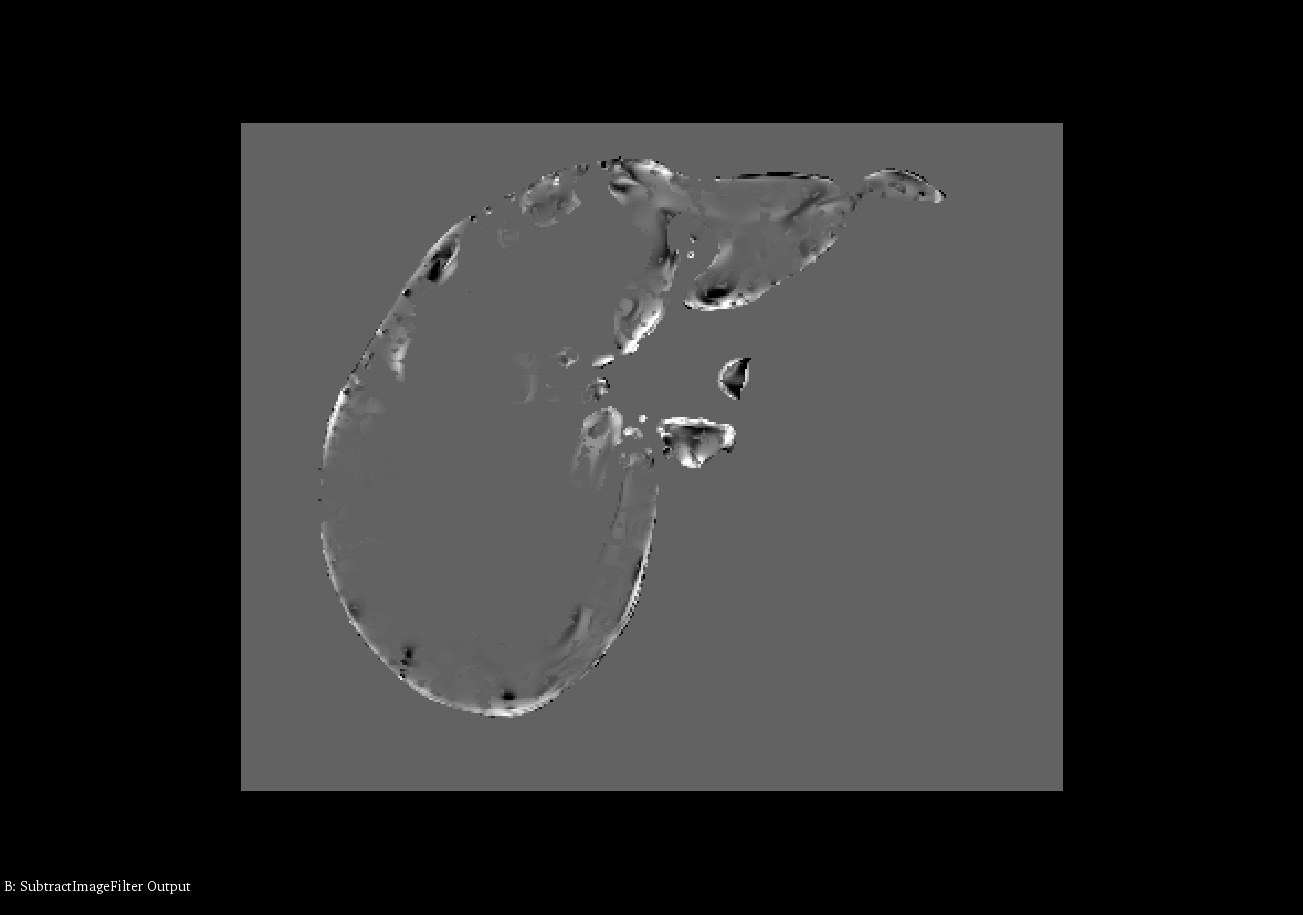
\includegraphics[height=3cm]{Images/output_masking_diff.png}
  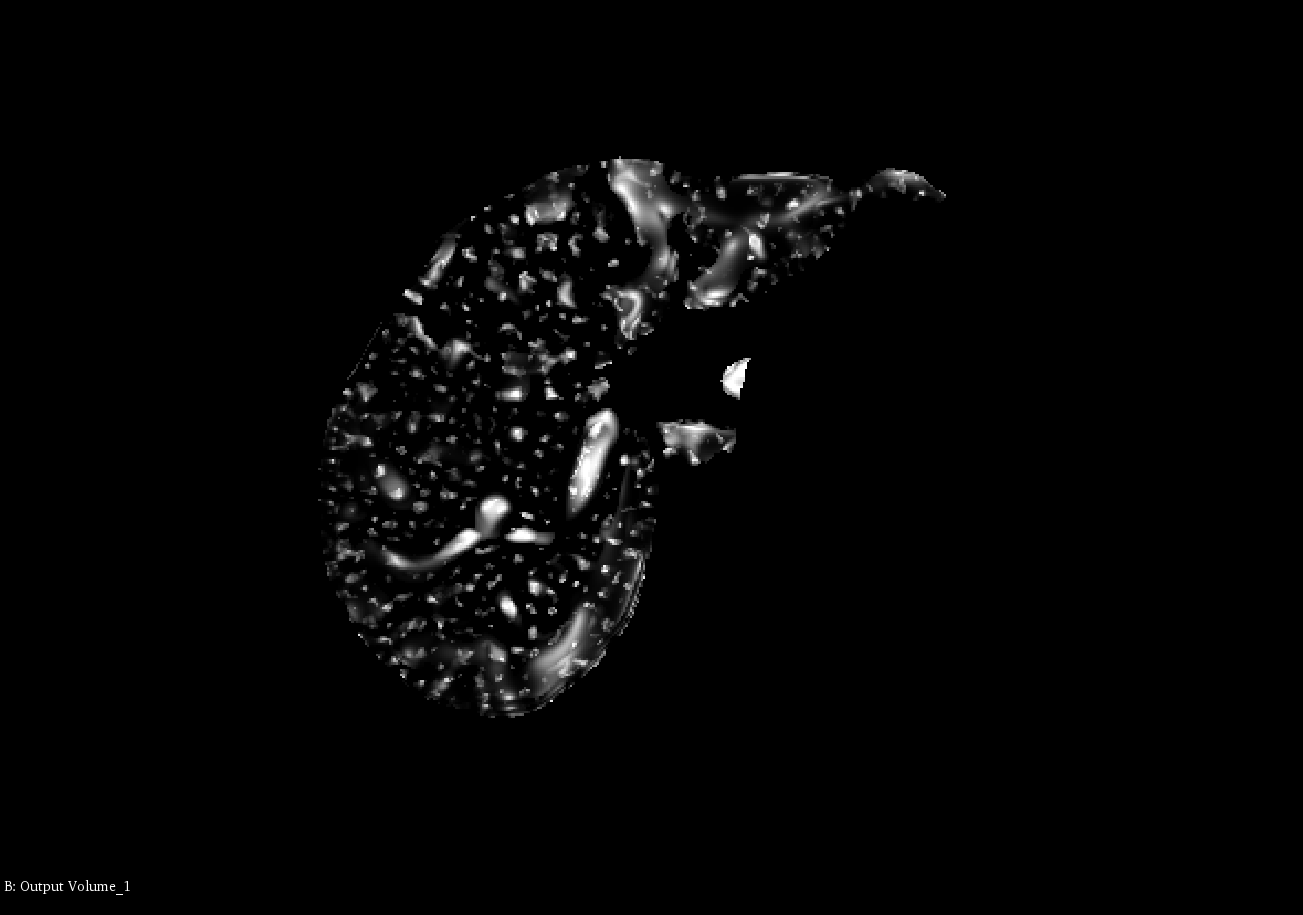
\includegraphics[height=3cm]{Images/output_unmasked.png}
  \label{fig:mask_intensity_profile}
  \caption{rehaussement avec masque en amont (gauche) et masque en aval (droite). La différence des deux masques est visible au centre. Le masque exacerbe la démarcation}
\end{figure}

De plus, on se heurte à un problème pour les filtres à information globale. On peut en effet classer les filtres de rehaussement en deux catégories. Les filtres à seule information locale et les filtres à information locale et globale. Les filtres à information locale ne considèrent le rehaussement que par rapport à des mesures effectuées dans un voisinage local. Ce voisinage est défini par la taille de la gaussienne pour les méthodes à espace d'échelles gaussien et par la taille de l'élément structurant pour les méthodes à base de morphologie. Les filtres à information locale sont Frangi, Sato, RORPO, OOF.

Les filtres à information globale sont Meijering, Jerman et Zhang. Meijering et Jerman/Zhang nécessitent respectivement la plus faible et la plus grande valeur propre de la zone sur lequel est appliqué le rehaussement. Le pré-filtrage de Zhang nécessite lui aussi une information globale puisque son pré-filtrage repose sur la classification de l'ensemble des pixels de la zone de rehaussement. Dans le cas de ces filtres, une implémentation naïve des masques à un impact critique sur le résultat du rehaussement. En effet, une image de l'abdomen contient aussi les os de la cage thoracique qui possèdent une intensité largement supérieure aux vaisseaux du foie. Dans le cas d'un filtre à information globale comme le filtre de Jerman, la mesure de rehaussement sera pondérée par les valeurs propres maximales de l'image, donc celle des os, et non celles des vaisseaux. 

Une stratégie de masque a donc été choisie spécifiquement pour chaque masque. Ainsi pour Frangi, Sato, OOF, RORPO le masque est appliqué après le rehaussement, cela afin de limiter l'introduction de faux gradients liés au masque.

Nous avons implémenté nous même les filtres de Jerman, Meijering et Zhang nous permettant d'avoir un contrôle plus fin sur l'étape d'application du masque. Afin de combiner les deux propriétés de limitation du temps de calcul et de non-introduction de bordures nettes artificielles, l'opération de masque est introduite entre le calcul de la matrice hessienne et le calcul de ses valeurs propres. Ne sont calculées les valeurs propres que des pixels appartenant au masque. On obtient ainsi le meilleur entre masque en amont et masques en aval.

\begin{figure}
  \centering
  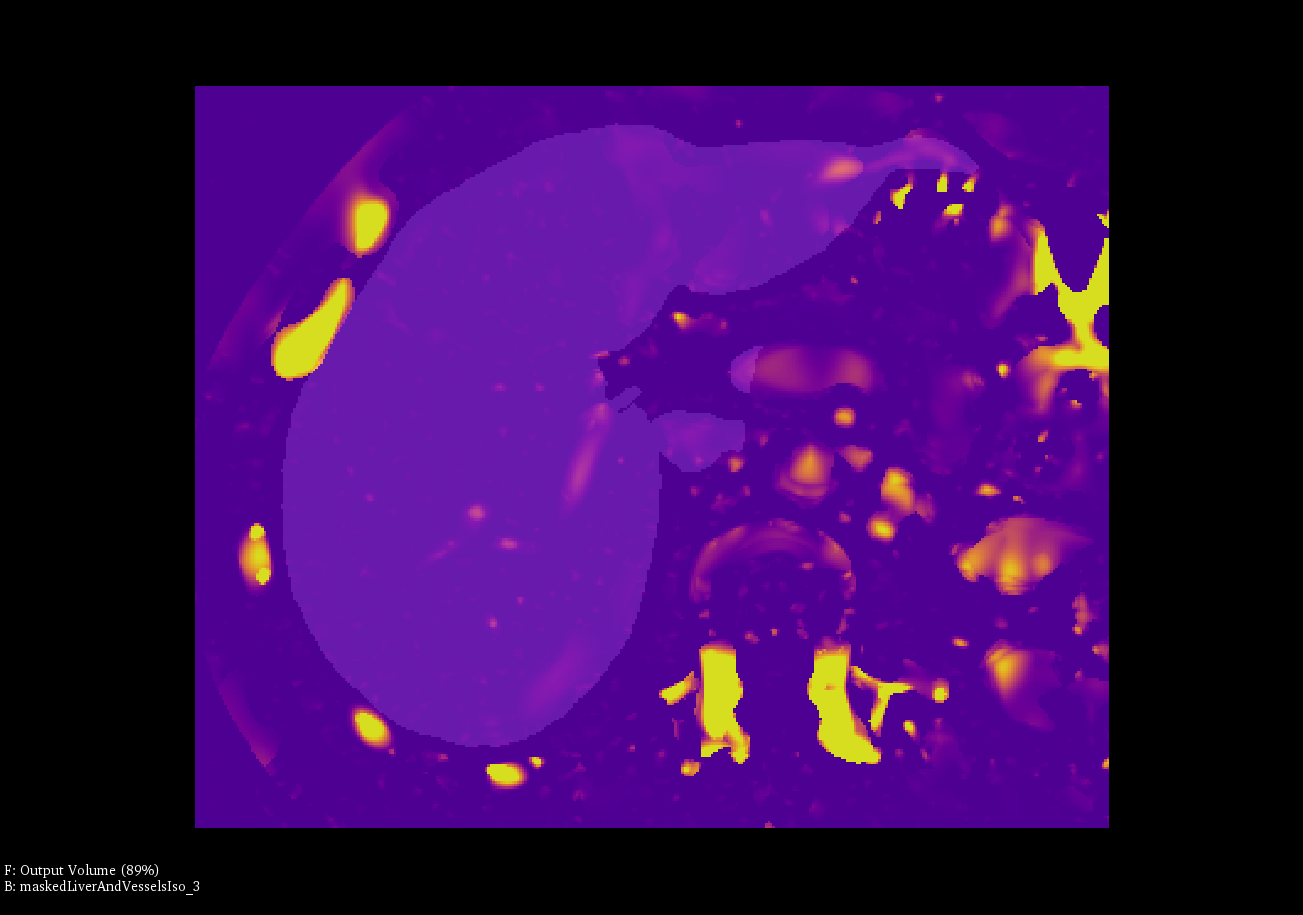
\includegraphics[height=4cm]{Images/globInfo_noM_glob.png}
  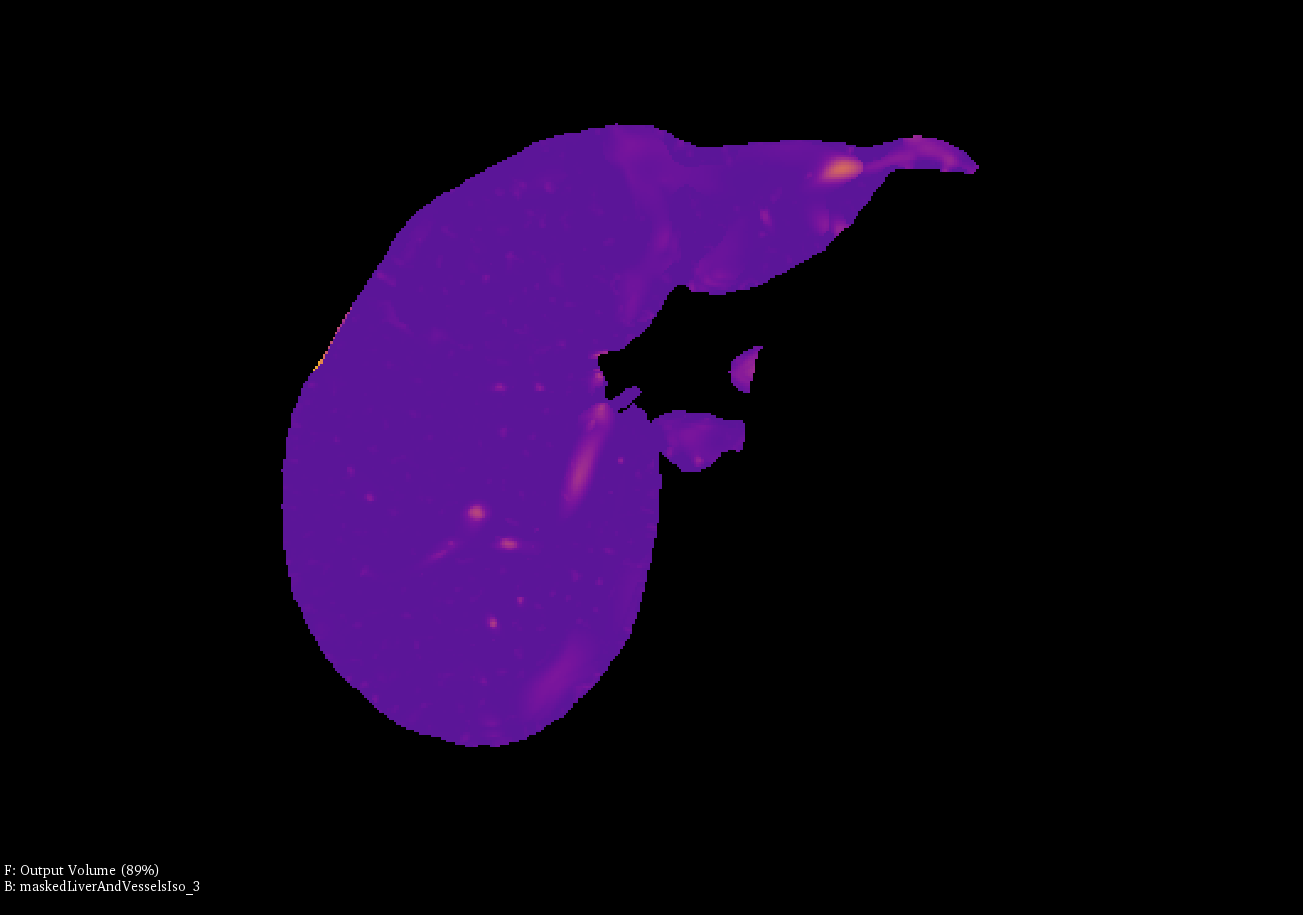
\includegraphics[height=4cm]{Images/globInfo_noM_loc.png}
  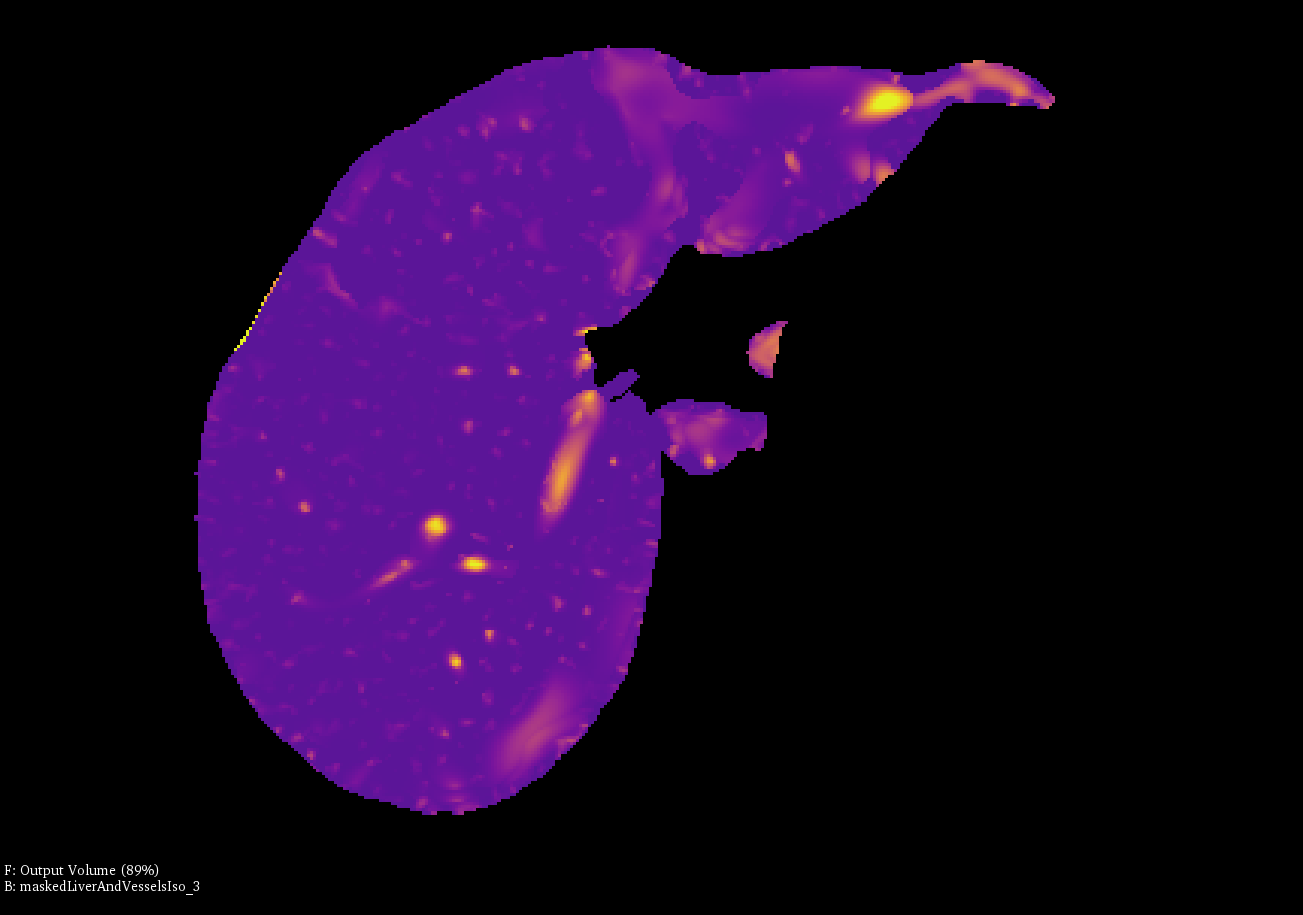
\includegraphics[height=4cm]{Images/globInfo_M_loc.png}
  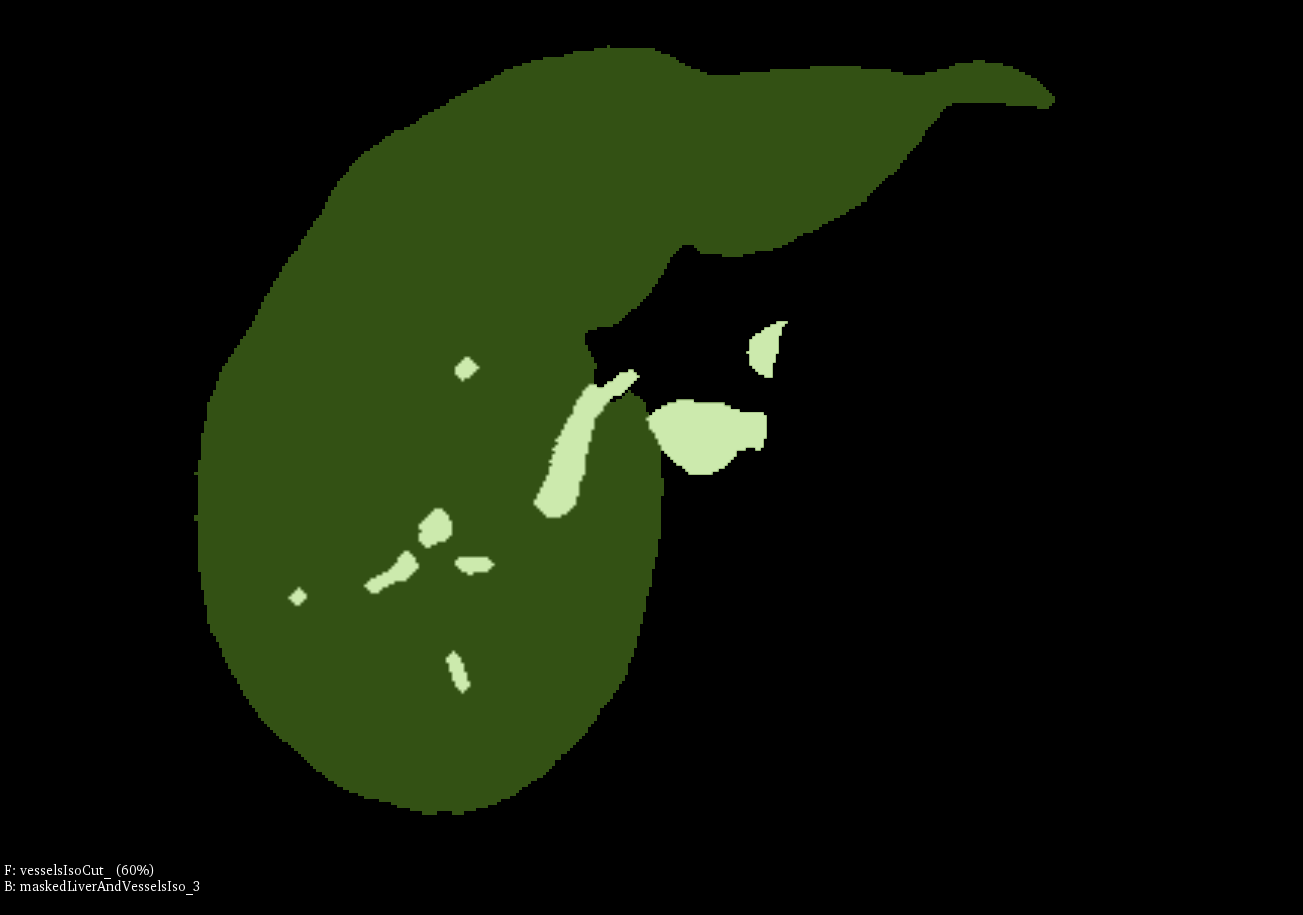
\includegraphics[height=4cm]{Images/globInfo_GT.png}
  \label{fig:smart_mask_effect}
  \caption{Filtre de Jerman appliqué sans prise en compte du masque (1ère ligne). Les structures extérieures perturbent le rehaussement des vaisseaux. Filtre de Jerman avec prise en compte du masque (2nd ligne). Les deux filtrages ont été réalisés avec les mêmes paramètres.}
\end{figure}

\begin{figure}[!t]

    \centering
    %\resizebox{\linewidth}{
      
  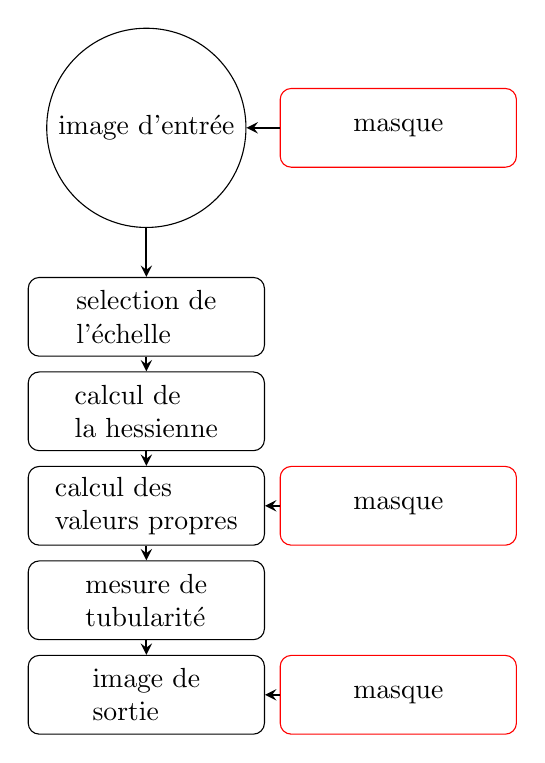
\begin{tikzpicture}[node distance=1.2cm]
    \node (input)[cNode] {image d'entrée};
    \node (scale_selection)[capNode, below of=input,align=left,yshift=-1.2cm] {selection de \\ l'échelle};
    \node (hessian)[capNode, below of=scale_selection,align=left] {calcul de \\ la hessienne};
    \node (EV)[capNode, below of=hessian,align=left] {calcul des \\ valeurs propres};
    \node (vesselness)[capNode, below of=EV,align=left] {mesure de \\ tubularité};
    \node (output)[capNode, below of=vesselness,align=left] {image de \\ sortie};

    \node (p1)[capNodeRed,right of=input,xshift=2cm]{masque};
    \node (p2)[capNodeRed,right of=EV,xshift=2cm]{masque};
    \node (p3)[capNodeRed,right of=output,xshift=2cm]{masque};
    
    \draw [arrow] (input) -- (scale_selection);
    \draw [arrow] (scale_selection) -- (hessian);
    \draw [arrow] (hessian) -- (EV);
    \draw [arrow] (EV) -- (vesselness);
    \draw [arrow] (vesselness) -- (output);

    \draw [arrow] (p1) -- (input);
    \draw [arrow] (p2) -- (EV);
    \draw [arrow] (p3) -- (output);

    %\draw [arrow] (bestScaleParameter) -| node[anchor=east]{}([shift={(1.3cm,0mm)}]bestScaleParameter.east)|-([shift={(0mm,-1mm)}]computeParams2.west);
  \end{tikzpicture}
%}
\caption{Emplacements possibles pour masquer la réponse.}
\label{FIG:masks_posible_location}
\end{figure}

Zhang est le filtre le plus complexe, avec une étape de prétraitement avec un K-moyenne paramétrant un filtrage par sigmoïd et la mesure de rehaussement. Dans la méthode originale, le nombre de classes du K-moyenne est défini par rapport à des images masquées. Ce K-moyenne est donc appliqué sur l'image globale masquée (fond mis à 0) avant le filtrage par sigmoïd. Ensuite la même stratégie de masquage que Jerman et Meijering est utilisé. Le K-moyenne classique est une opération coûteuse, en particulier lorsqu'il est effectué sur un volume 3D. Afin d'éviter un surcoût, nous avons utilisé un K-moyenne à partir d'un quadtree qui réduit significativement le temps de calcul de cette étape.

Les 7 filtres sont implémentés en C++ et reposent sur la librairie ITK. Ceux-ci sont implémentés sont forme de CLI (command line interface) indépendants du cadre du banc de test et peuvent être utilisés indépendamment de celui-ci. Cela veut aussi dire que n'importe quel nouveau filtre respectant l'interface définie dans le benchmark (c'est-à-dire une entrée, une sortie et un masque optionnel) peut être ajouté de manière transparente à celui-ci.

\section{Pré-traitements des jeux de données}
\label{sec:Benchmark:traitement_des_données}

Notre objectif premier d'évaluer les filtres de rehaussement dans des images d'IRM du foie a dû être revu suite à un manque de données avec segmentation des vaisseaux (cf. Chapitre 1). Nous avons donc réorienté notre axe de travail sur l'évaluation des filtres sur des jeux de données publiques.

Dans un premier temps, nous avons utilisé la base de l'Ircad puis nous avons cherché à compenser l'absence de modalité IRM grâce à des données synthétiques issues du logiciel VascuSynth \cite{Hamarneh2010_VascuSynth}, données que nous avons modifiées. Le traitement de ces données a connu deux itérations successives permettant de raffiner l'analyse des filtres de rehaussement.

Nous avons utilisé dans un deuxième temps ajouté une troisième base d'IRM réelle du cerveau Bullitt, elle aussi publique afin de diversifier nos résultats.

\subsection{Traitement des données réelles}

La résolution d'une image est le nombre d'échantillons/de voxels, utilisés pour représenter une taille physique. Pour une même distance physique, plus le nombre d'échantillons sur cette distance, et donc le nombre de voxels, est élevé plus la résolution de l'image est élevée. Contrairement aux images classiques les images issues d'IRM et de TDM, les voxels sont ont des résolutions anisotropiques. Comme montré dans le chapitre 2, l'acquisition des images d'un patient se fait de manière itérative. Afin que les temps d'acquisitions ne soient pas trop long, la résolution de l'axe Z, l'axe tête-pied, est souvent plus faible que la résolution axiale (axes X et Y). Dans le meilleur des cas, celle-ci correspond au minimum au double de la résolution axiale dont les valeurs se situent en dessous du millimètre, dans le pire des cas, elle peut être bien plus élevée et atteindre jusqu'à 5mm.

Un ré-échantillonnage est nécessaire afin de faire fonctionner la plupart des algorithmes de traitement d'image. En effet ceux-ci sont développés pour fonctionner sur des grilles discrètes cubiques, isotropes et non des parallélépipèdes anisotropes. Par exemple, pour le calcul d'une distance euclidienne entre deux pixels, on s'attend à ce que la distance parcourue soit la même, peu importe la direction de la ligne séparant ces deux points. Une pondération des filtres par la résolution des images serait trop complexe à mettre en place. Il est donc plus simple d'agir directement sur les données.

L'échantillonnage consiste à considérer un signal continue sur lequel on va relever des échantillons à intervalles réguliers. Les valeurs de ces échantillons constituent ensuite les valeurs des voxels des images. Le ré-échantillonnage consiste à modifier l'intervalle et le nombre de ces échantillons. Pour obtenir un ré-échantillonnage, on passe par des calculs d'interpolation entre les échantillons afin de reconstruire implicitement l'image continue.

\begin{figure}
  \centering
  
\includegraphics[height=3cm]{Images/img_required.jpg}
  
\includegraphics[height=3cm]{Images/img_required.jpg}
  
\includegraphics[height=3cm]{Images/img_required.jpg}
  \caption{illustration de l'échantillonnage}
\end{figure}

Nous avons exploré plusieurs manières de ré-échantillonner les images pour les rendre isotropes. Notre premier type d'échantillonnage a été d'échantillonner l'image à une résolution de 1 mm pour chaque axe. Ce ré-échantillonnage a l'avantage de réduire la taille des images tout en rendant les voxels cubiques. En pratique, on perd en résolution spatiale axiale et on gagne en résolution spacial dans l'axe Z dégradant légèrement la géométrie. Cet échantillonnage permet de limiter grandement la taille mémoire des volumes en réduisant significativement le nombre de voxels. Cela permet de faire tenir le benchmark dans des ordinateurs avec des mémoires RAM inférieures à 10 Go. En effet, l'utilisation d'un cadre multi-échelles fait exploser rapidement la mémoire nécessaire. Cette technique permet donc de limiter cet effet.

La perte de résolution peut toutefois s'avérer un problème, car elle endommage la géométrie des vaisseaux. Les plus petits vaisseaux ont en effet une épaisseur proche de la résolution initiale. Afin de ne perdre aucune information, nous avons ré-échantillonné les images à leur résolution la plus élevée, c'est-à-dire la résolution axiale. Les détails sont ainsi conservés et les voxels rendus cubiques. Cependant, augmenter la résolution pour une même taille d'image revient à augmenter le nombre de voxels de celles-ci. On obtient donc des images significativement plus lourdes que les images originales, car l'augmentation de la résolution revient à augmenter le nombre de voxels de l'image. Cela impacte à la fois la mémoire nécessaire ainsi que le temps de calcul des filtres.

\begin{figure}
  \centering
  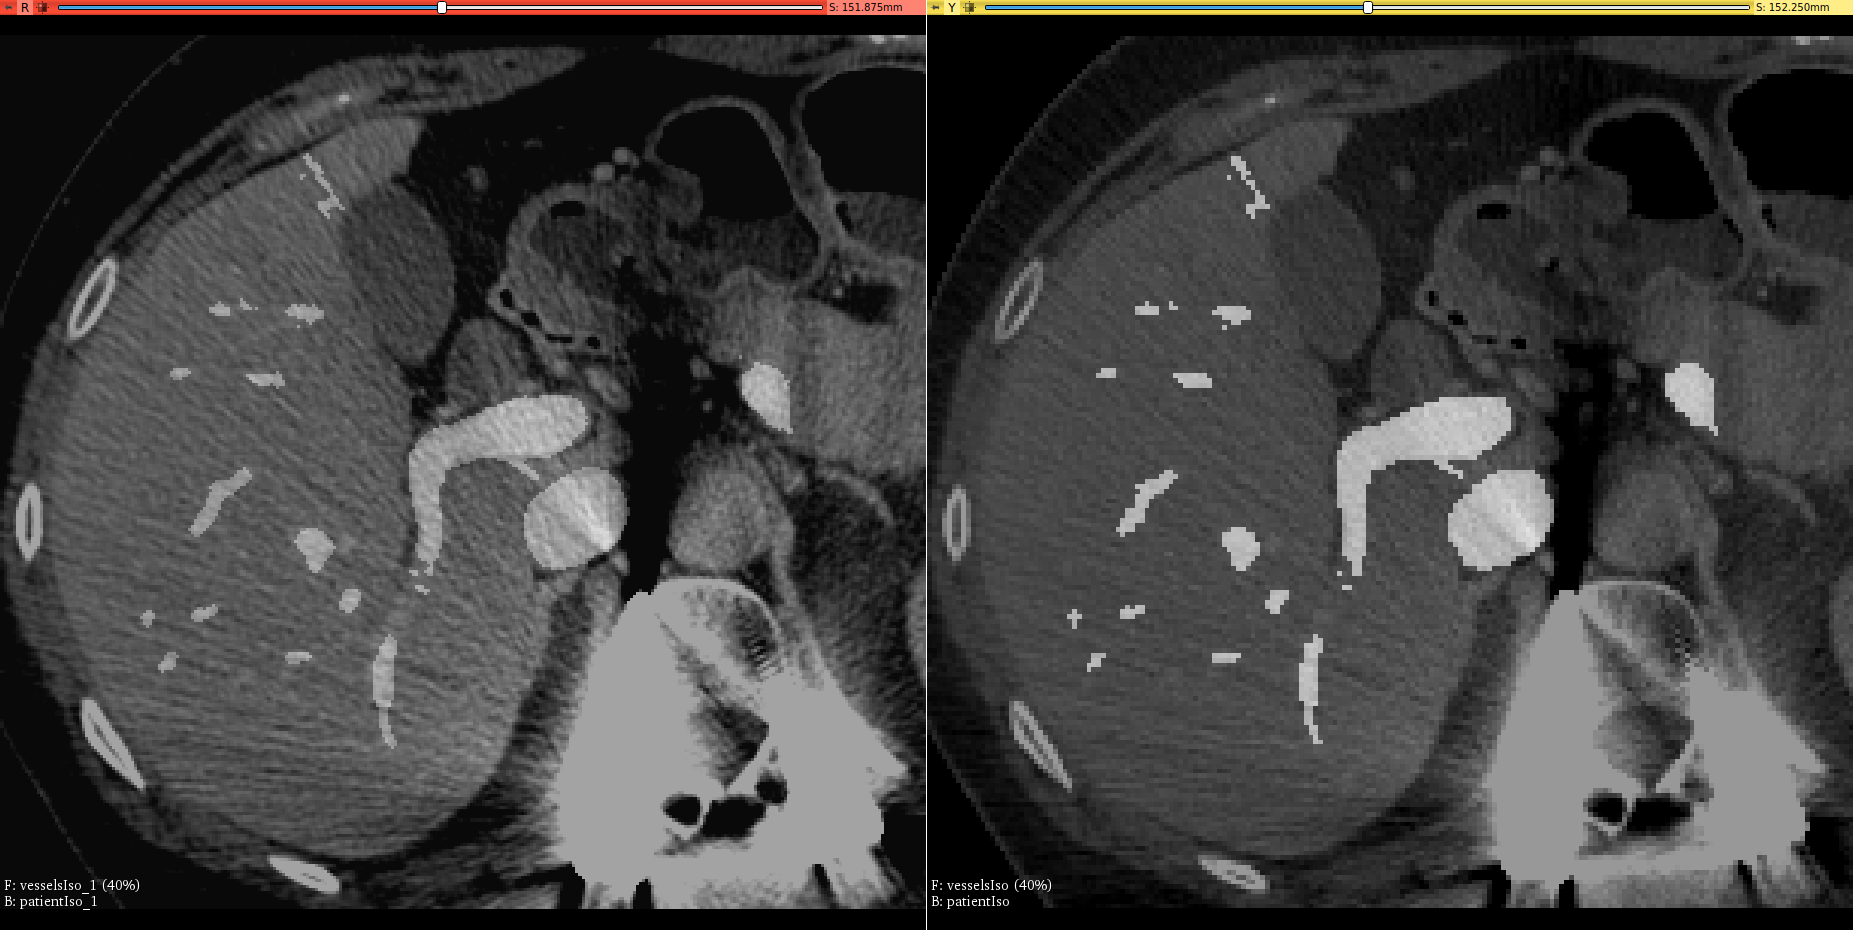
\includegraphics[height=6cm]{Images/resolution_comparison.png}
  \caption{différence de géométrie liée aux deux stratégies d'échantillonnage. L'image de résolution plus élevée contient 4x plus de voxels ($~27M$) que l'image basse résolution ($~6.6M$) mais la géométrie des vaisseaux est mieux préservée.}
\end{figure}

Afin de mitiger l'augmentation des tailles d'images, nous les avons recadré pour supprimer le maximum de voxels inutiles, c'est-à-dire ceux en dehors du masque de l'organe. Pour ce faire, nous avons redimensionné les images à la taille de la boite englobante du masque de l'organe en incluant une bordure de sécurité de 15 voxels. Selon les bases, la récupération de la boite englobante peut nécessiter dans un premier temps une analyse en composante connexe afin de récupérer la boite englobante la plus grande. La consistance des masques des organes n'est pas toujours assurée et des pixels déconnectés peuvent être présents dans les images de masques.

On limite ainsi la taille des images au maximum sans perdre d'informations utiles. Nous avons ainsi obtenu un gain de \todo{valeur à calculer} en moyenne sur le nombre de pixels.



Les images en niveau de gris ont été ré-échantillonné à l'aide d'une interpolation à base de B-spline d'ordre 2.
Les images binaires ont été ré-échantillonné à l'aide d'une interpolation à base de plus proches voisins afin de conserver le caractère binaire des images.

Pour la base de données Bullitt, les images d'IRM sont des images destinées à la recherche et sont particulièrement de bonne qualité. Une fois un masque du cerveau obtenu, il est très facile de récupérer les vaisseaux grâce à un simple seuillage. Nous avons donc complexifié ces données en renforçant les artefacts IRM en ajoutant une gaussienne de pondération des intensités et un niveau de bruit ricien plus fort $\sigma=4$. 

\subsection{Génération de données synthétiques}

Nous avons à notre disposition la base de donnée de l'Ircad pour le foie. Cependant, cette base est acquise par tomodensitométrie. Hors, cette modalité a été relativement bien explorée dans la littérature et l'un des objectifs initiaux était l'évaluation du rehaussement dans des images IRM. Le manque de données IRM annotées nous oblige à nous tourner vers des données synthétiques. Les bases de données synthétiques ont l'inconvénient d'être moins réalistes que les bases naturelles. Elles présentent cependant l'avantage d'un environnement complètement contrôlé par l'utilisateur et permettent d'obtenir des vérités terrains au pixel près.

VascuSynth, présenté dans le Chapitre 2, permet de définir des images synthétiques. Le logiciel permet de créer un arbre vasculaire en précisant le nombre d'extrémités de celui-ci, une carte d'oxygénation qui contrôle les zones de propagation de l'arbre et une suite de paramètres physiologiques comme la pression sanguine.

\begin{figure}
  \centering
  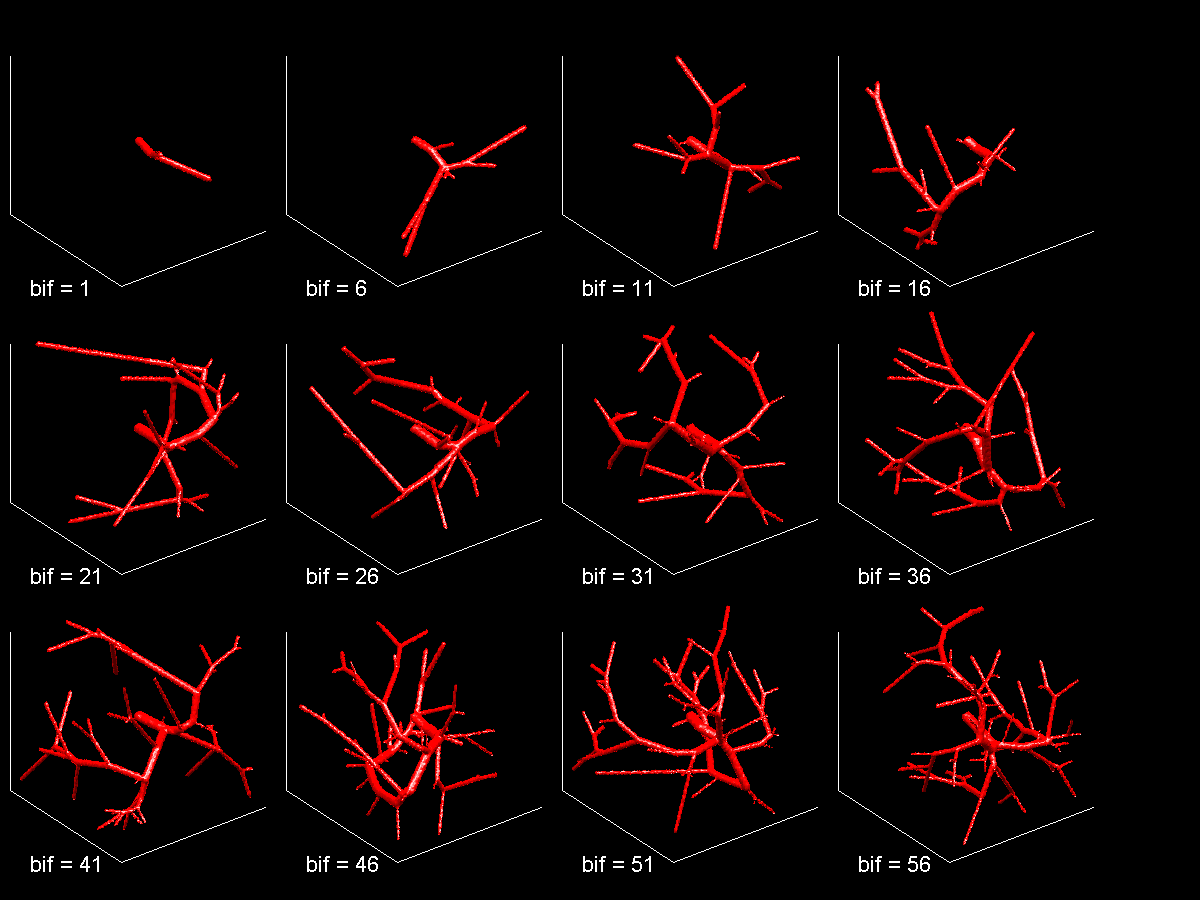
\includegraphics[height=5cm]{Images/snapVascu.png}
  \label{fig:smart_mask_effect}
  \caption{Image d'illustration des vaisseaux de la base VascuSynth disponible avec le jeu de données. Le jeu de données présente différents nombres de bifurcations.}
\end{figure}

Nous avons utilisé dans nos expériences la base de donnée VascuSynth 2013 disponible sur le site de VascuSynth. Cette base est composée de volumes avec des arbres vasculaires de différentes tailles sur un fond nul. VascuSynth produit des images en niveau de gris de 0 à 255. L'intensité des vaisseaux est relativement forte (autour de 230, à vérifier) et n'est pas homogène. L'intensité des vaisseaux décroit légèrement sur les bords de ceux-ci et est un peu plus faible pour les petits vaisseaux.

On peut obtenir une vérité terrain au pixel prêt en binarisant ce volume initial.

Nous avons voulu transformer ces images de manière à imiter l'apparence de l'IRM appliquée au foie. Cette génération de volumes IRM a connu plusieurs itérations que nous détaillons ici.

% intensité du foie
Nous avons généré nos images en 4 étapes.
Premièrement, nous avons redéfini la game d'intensité des vaisseaux. En effet, ceux-ci étant d'intensité trop élevée, ils ne permettent pas l'ajout de bruit et d'éléments additifs sans saturer les voxels et perdre l'information des vaisseaux. Une simple mise à l'échelle des intensités et une translation suffisent. Ensuite, nous avons ajouté un fond homogène d'intensité égale à l'intensité minimale des vaisseaux. En effet, dans l'imagerie du foie avec agent de contraste, les vaisseaux sont en principe d'intensité supérieure ou égale à l'intensité des tissus.

\begin{figure}
  \centering
  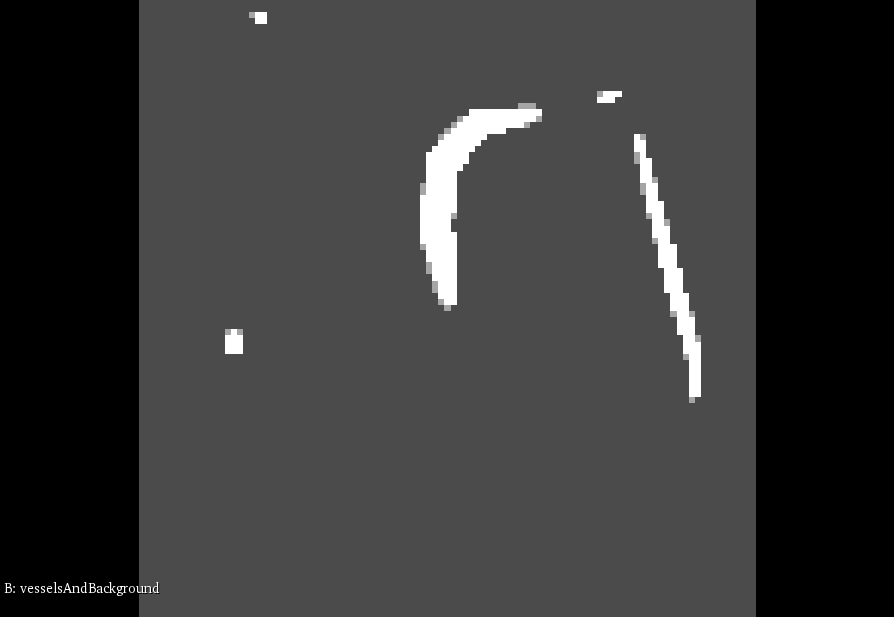
\includegraphics[height=3cm]{Images/2D_VB.png}
  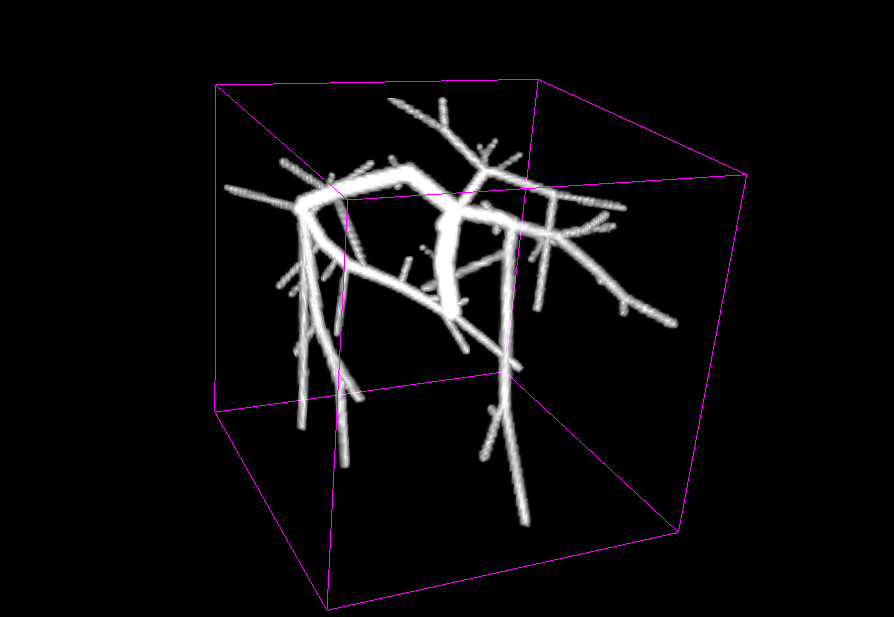
\includegraphics[height=3cm]{Images/3D_VB.png}
  \label{fig:VB}
  \caption{Vaisseaux et fond. Le fond est d'intensité égale à l'intensité minimale des vaisseaux.}
\end{figure}

Dans un premier temps, nous n'avons pas réalisé de changement d'intensité le long des vaisseaux. Nous aurions pu faire décroitre l'intensité des vaisseaux en partant de la base de l'arbre et en faisant décroitre la valeur des voxels des vaisseaux par propagation de proche en proche. Cependant, les variations d'intensités dans les vaisseaux est un processus plus complexe qu'une simple baisse linéaire de l'intensité. Cette variation dépend des propriétés de mécaniques des fluides de l'agent de contraste dans le sang ainsi que de la géométrie des vaisseaux.

L'intensité du fond a été fixé à 50 et l'intensité maximale des vaisseaux à 100. 

Nous avons ensuite voulu exploiter les différences d'intensité entre les tissus de même nature. Nous émulons cette non-homogénéité illustrée dans le Chapitre 2, par la création d'un volume dans lequel 3 gaussiennes de taille $\sigma=40$, sont tirés dans l'espace de manière aléatoire et additionnées dans un même volume avant d'être réajusté dans des intensités comprises entre 50 et 100. Un opérateur max est ensuite utilisé entre le volume contenant les vaisseaux et les gaussiennes d'intensité similaire. L'opérateur max avait été choisi de manière à émuler l'intensité des vaisseaux les plus fins qui se fondent dans l'intensité des tissus environnant.

\begin{figure}
  \centering
  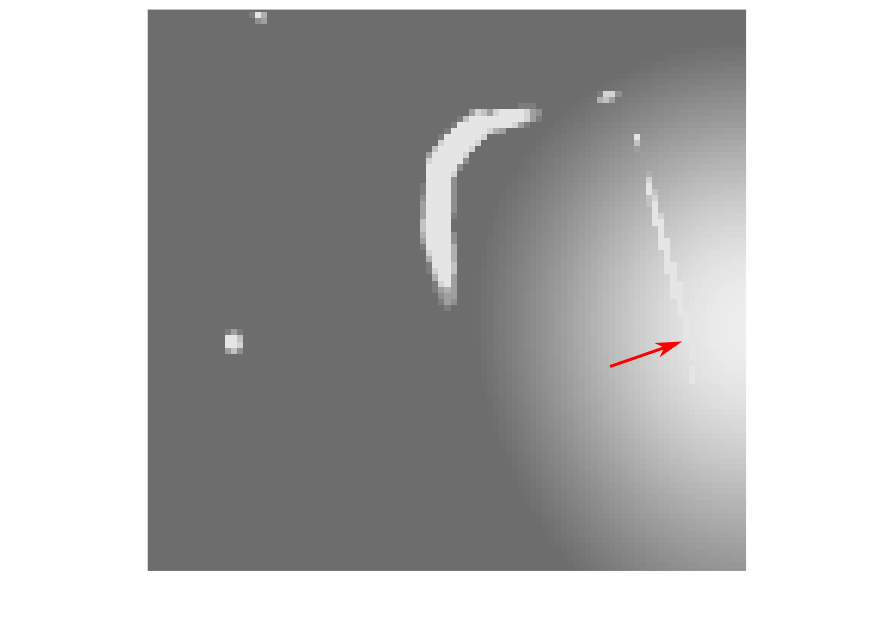
\includegraphics[height=3cm]{Images/2D_VBI.png}
  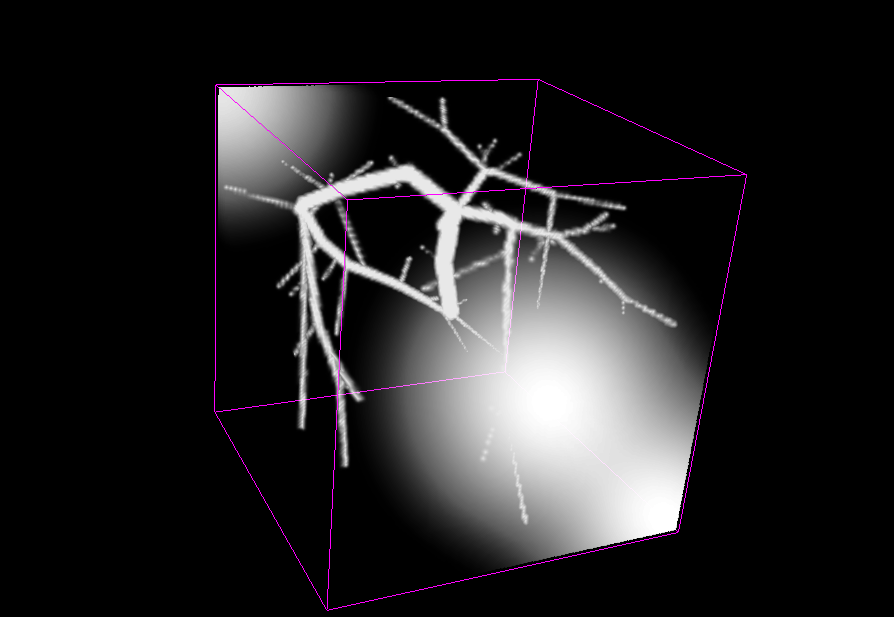
\includegraphics[height=3cm]{Images/3D_VBI.png}
  \label{fig:VBI}
  \caption{Vaisseaux avec illumination. Certains vaisseaux disparaissent dans les tissus.}
\end{figure}

Nous avons ensuite ajouté du bruit ricien qui est un bruit multiplicatif spécifique à l'IRM. Par contraste, la plupart des expériences sur bases de données synthétiques appliquent une mixture de bruit de poisson et gaussien caractéristique du bruit présent en tomodensitométrie.

\begin{figure}
  \centering
  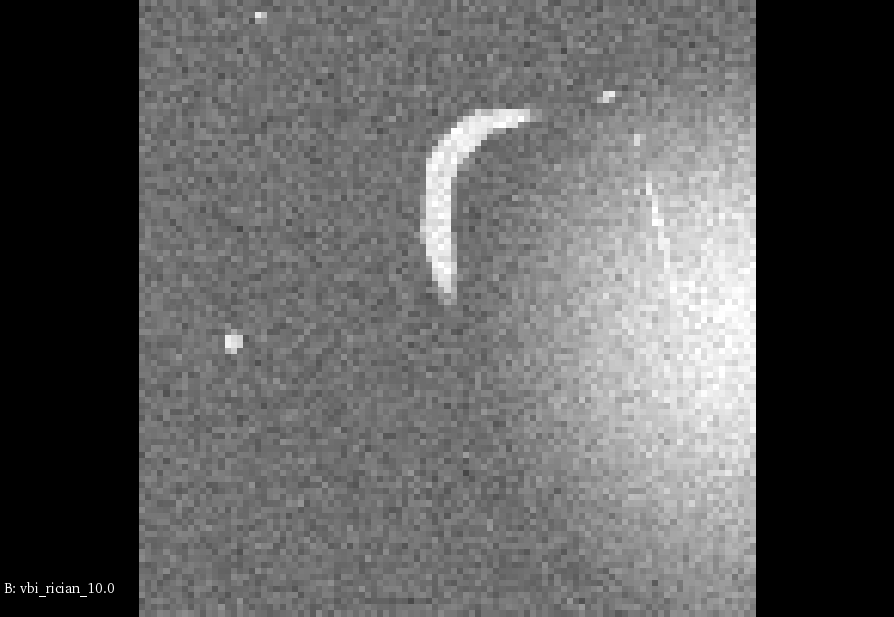
\includegraphics[height=3cm]{Images/2D_VBIR10.png}
  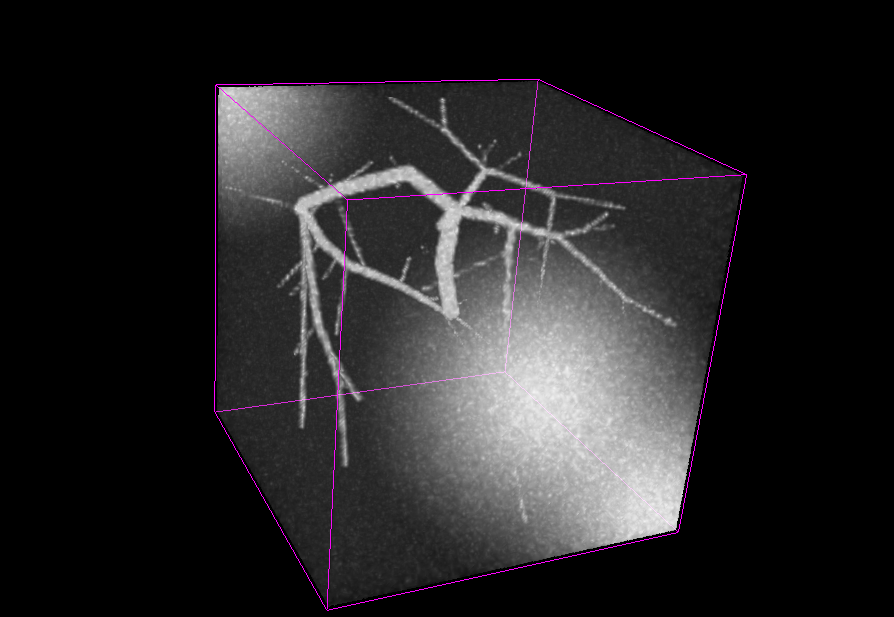
\includegraphics[height=3cm]{Images/3D_VBIR10.png}
  \label{fig:2D_VB}
  \caption{Vaisseaux et fond. Le fond est d'intensité égale à l'intensité minimale des vaisseaux.}
\end{figure}

Cette première itération était une bonne approximation. Cependant celle-ci souffre de plusieurs limitations. Premièrement la dynamique d'intensité est établie de manière visuelle. De même pour le bruit ricien. Deuxièmement, le max effectué entre les images et les vaisseaux fait disparaitre des vaisseaux qui sont tout de même présents dans la vérité terrain. On introduit ainsi une baisse artificielle des performances puisque qu'aucun filtre n'est en réalité capable de rehausser ces structures invisibles. En vérité, la plupart des vaisseaux peuvent être récupérés par un seuillage simple lorsque le niveau de bruit ne recouvre pas le signal. Ce problème est notamment visible à travers les MIP puisque l'intégralité des vaisseaux sont visibles quand ils ne sont pas recouverts par des blobs gaussiens.

Dans une deuxième itération, nous avons revu le processus de création de ces volumes.

Les vaisseaux sont toujours mis à l'échelle et le fond toujours définit comme l'intensité minimale des vaisseaux. Cependant, la plage d'intensité des vaisseaux est cette fois ci définit par rapport à des mesures faites sur des bases de données réelles. Pour cela nous avons réalisé des mesures manuelles sur des images d'IRM. Sur quelques volumes (de mémoire 5-6, retrouver les valeurs), une dizaine de coupes axiales ont été réalisée sur lesquelles ont été annotés deux masques, un masque des tissus et un masque des vaisseaux. Pour chaque type de masque, nous avons calculé la moyenne et l'écart type de l'intensité des vaisseaux et des tissus du foie. La moyenne des tissus du foie est de 1273 contre 1400 pour celle des vaisseaux. L'écart type respectif des tissus est de 144 et de 189 pour les vaisseaux pour des volumes avec une dynamique d'intensité comprise entre 0 et 3000. En exprimant ces quantités proportionnellement à la dynamique de VascuSynth ($[0,255]$), on obtient $\mu=108 \pm 12$ pour les tissus du foie et $\mu=119 \pm 16$. En pratique le différentiel entre la moyenne des vaisseaux et des tissus est faible, alors qu'elle est localement plus importante. Cet écart est aussi trop faible pour obtenir des gaussiennes discrètes avec un sigma élevé de bonne qualité dans les étapes suivantes. Nous avons donc considéré l'intensité des vaisseaux comme la somme de leur moyenne et de l'écart type. Nous augmentons ainsi la dynamique tout en restant cohérent avec les mesures physiques.

Nous avons ensuite introduit deux filtres d'inhomogénéité : Un premier afin de diversifier le profil d'intensité des vaisseaux et un second pour diversifier l'intensité globale de l'image. Dans le premier cas, celle-ci essaie d'approcher les variations d'intensités liées à l'agent de contraste. Dans le second cas, cette modification a été faite pour que le jeu de données soit résistant à une segmentation par simple seuillage. L'objectif est alors que localement les vaisseaux restent des maxima locaux, mais que ceux-ci soient d'intensité plus faible que des tissus du foie situés à l'autre bout du volume.

Pour cela l'algorithme de génération change légèrement. Pour le changement d'intensité dans les vaisseaux, on utilise un masque avec des gaussiennes tirées aléatoirement, ces gaussiennes sont pondérées de manière à faire diminuer l'intensité des vaisseaux au maximum de $30$ pour cent par rapport à leur intensité initiale. Les gaussiennes étant tirées dans l'espace entier de l'image on obtient des variations non linéaires le long des vaisseaux.

Cette étape est réalisée en premier, avant l'étape de mise à l'échelle et de translation des vaisseaux et l'ajout du fond.

Ensuite une pondération de l'ensemble de l'image est effectuée. Le principe est utilisé, mais cette fois-ci, la diminution touche au maximum $40$ pour cent de l'intensité originale des pixels.

Ensuite des artefacts gaussiens sont ajoutés pour venir perturber les filtres de rehaussement en introduisant des structures tubulaires, planaires ou en forme de blob. Pour cela, une dizaine d'éléments gaussiens avec un sigma aléatoire pour chaque axe de l'image sont introduits. Ces artefacts sont introduits de manière additive. Par conséquent l'introduction d'artefacts ne provoque aucune disparition de vaisseaux. Dans le pire des cas, un saut d'intensité est observé.

On obtient ainsi un jeu de test reproduisant 4 artefacts courants dans les images d'IRM.
 
\section{Construction des zones d'évaluation des filtres}

Pour évaluer la segmentation voxélique de manière précise, nous avons souhaité évaluer le rehaussement dans plusieurs régions. La première région est l'organe dans sa totalité. Cette région est celle choisis la plupart du temps pour la segmentation. L'étude de cette région pose plusieurs questions. Un filtre arrive-t-il à rehausser les vaisseaux sans rehausser d'autres éléments de l'image ? Dans quelle proportion ? Le rehaussement introduit-il de nouvelles structures ou artefacts ?

La seconde région d'intérêt concerne les vaisseaux et leur voisinage. Cette région nécessite la segmentation manuelle des vaisseaux par un expert. Elle permet de répondre à plusieurs questions. Quelle est la qualité du rehaussement des vaisseaux ? Les vaisseaux sont-ils rehaussés avec une taille supérieure ou inférieure à leur taille réelle ? Cette région peut être subdivisée en partitions en fonction de la taille ou de la hiérarchie des vaisseaux. On peut ainsi analyser quels types de vaisseaux sont les mieux rehaussés et dans quel contexte.

La troisième région d'intérêt concerne les bifurcations des vaisseaux. Ces zones sont particulières, car elles correspondent à une jonction des vaisseaux tubulaires. Dans ces zones, la géométrie n'est plus tubulaire et Le rehaussement peut donc y être affaibli. Cette perte de signal a été signalée dans de nombreuses publications en étant illustrée de manière visuelle sur des données synthétiques. Par contre, elle n'a, à notre connaissance, jamais été évaluée quantitativement.

% M global
Pour la zone d'intérêt des organes, celle-ci est relativement simple à obtenir à l'aide d'outils semi-automatiques comme les levels sets ou la croissance de région à partir de marqueurs placés à la main. La géométrie de la bordure des organes est la plupart du temps, simple et bien définie. Il peut cependant arriver que le mouvement du patient durant l'acquisition fasse fusionner des tissus, comme c'est souvent le cas entre le foie et l'estomac. Dans ce cas, une correction manuelle peut-être nécessaire.
% M vaisseaux
La construction des zones d'intérêts du voisinage des vaisseaux passe par l'utilisation des vérités terrains.
Pour la vérité terrain des vaisseaux, une première approximation peut-être obtenue par seuillage en profitant de leur profil d'intensité élevé, cependant la majeure partie des annotations doit être réalisée manuellement par un expert. Ces vérités terrains prennent généralement une heure pour un foie. Une paire de vue 2D et MIP 3D permettent de valider les annotations de manière simple et améliorent considérablement la qualité des annotations.
% M vaisseaux G - M - P
Pour obtenir une zone d'intérêt du voisinage des vaisseaux, On peut dilater la vérité terrain des vaisseaux. Nous avons dans un premier temps réalisé une dilatation globale. Cependant, celle-ci n'est pas forcément pertinente selon la taille des vaisseaux, puisque les gros vaisseaux se retrouvent avec une proportion vaisseaux/fond inférieure aux petits vaisseaux. De plus, afin d'avoir une information complémentaire sur le voisinage des vaisseaux, nous avons réalisé une partition par taille en 3 classes : Gros vaisseaux, correspondants au tronc porte du foie. Les vaisseaux de taille moyenne correspondant aux vaisseaux des premiers embranchements hépatiques et aux artères du cerveau, et enfin les petits vaisseaux correspondant aux vaisseaux aux extrémités des réseaux vasculaires.

Cette partition nécessite un traitement sur la vérité terrain originale. Celle-ci nécessite de labelliser chaque branche de vaisseaux en fonction de leur diamètre avant de les classifier dans trois sous labels.

\subsection{Masques globaux}

Les masques globaux du foie sont déjà disponibles dans le dataset de l'Ircad. Cependant, ils n'incluent pas le ou les premier(s) embranchement du tronc porte et la base de la veine cave légèrement à l'extérieur du foie. Ainsi lorsque l'on masque la vérité terrain des vaisseaux par le masque du foie, on produit une vérité terrain avec de nombreux vaisseaux déconnectés entre eux et des fragmentations de certaines vérités terrains. Ceci peut être problématique pour une analyse des composantes connexes après filtrage et binarisation. C'est aussi problématique pour l'évaluation de filtres nécessitant une graine d'initialisation, car les bases des veines est facilement identifiable. De plus, pour les médecins, il est plus simple de planifier une opération à partir d'un arbre vasculaire complet plutôt que des vaisseaux déconnectés.

Nous avons utilisé ces masques tels quels dans un premier temps avant de raffiner ceux-ci manuellement. Pour cela, nous avons réalisé une partition manuelle de la segmentation des vaisseaux en dehors du foie avant de fusionner cette partition avec le masque du foie.

\begin{figure}
  \centering
  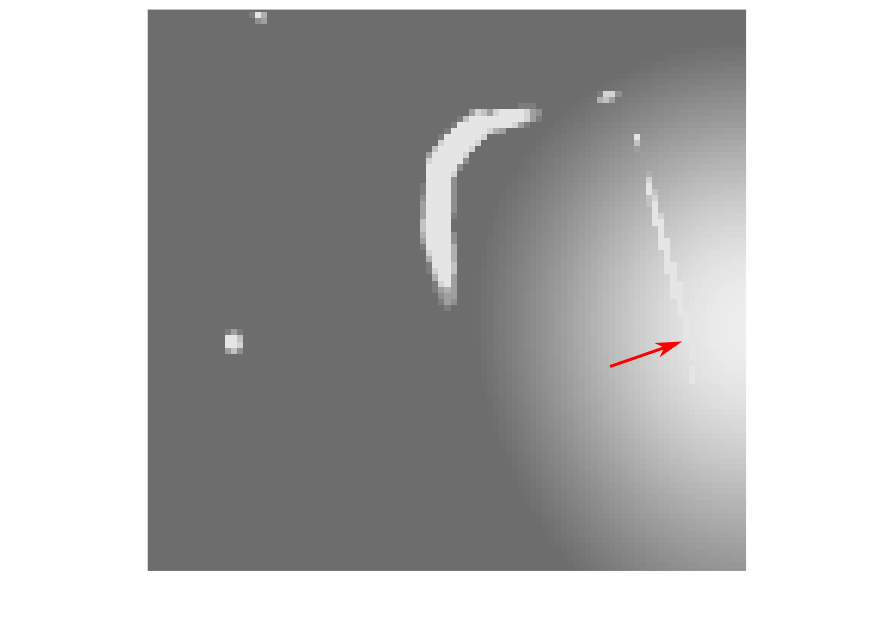
\includegraphics[height=3cm]{Images/2D_VBI.png}
  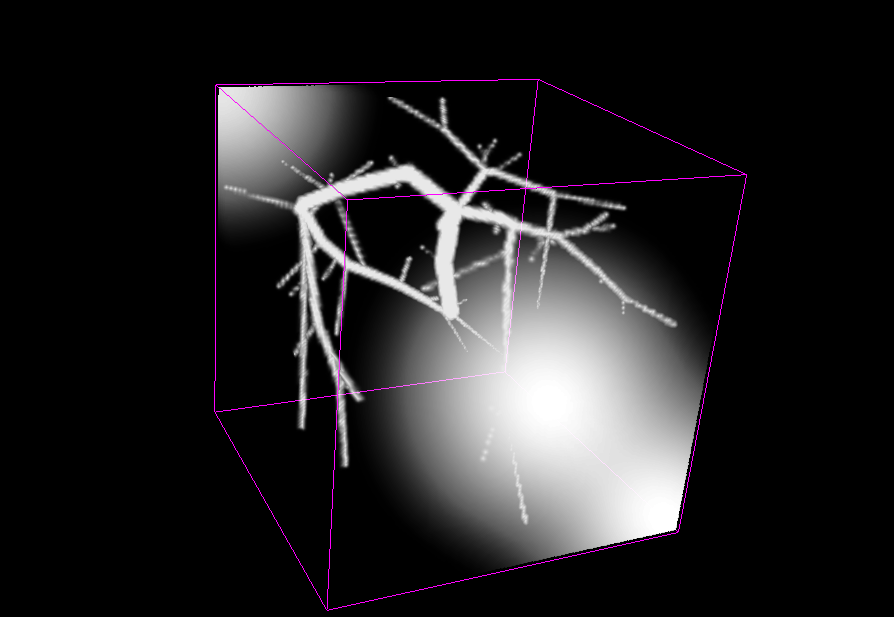
\includegraphics[height=3cm]{Images/3D_VBI.png}
  \label{fig:masques_globaux_ircad}
  \caption{A gauche, masque à l'itération 1 et segmentation masquée morcelée. A droite, masque à l'itération 2 comprenant les veines portes.}
\end{figure}

Pour le jeu de données issu de VascuSynth, il n'y a pas d'organes à proprement parlé. Le masque global est donc un masque recouvrant l'image entière. Nous aurions pu créer un masque artificiel et simuler des bordures d'organes, cependant cette problématique est déjà couverte par les deux autres bases de données. De plus, ceci nous permet d'évaluer la qualité du rehaussement sans la présence d'artefacts de bordure.

Pour Bullitt, nous avons été confrontés à deux problèmes. Le premier est qu'il n'y avait pour cette base pas de masques du cerveau. Ces masques ont dû être créés manuellement pour les 33 volumes utilisés. Deuxièmement, nous avons dû faire face à un problème d'annotations. En effet, les annotations augmentées par un système semi-automatiques sont inconsistantes. En effet, de larges veines en périphérie du cerveau ne sont pas annotées. Celles-ci auraient été manifestement visibles lors du rehaussement et auraient influencé négativement les résultats présentés dans le chapitre suivant. Nous avons donc choisi de réduire le masque du cerveau de manière à ignorer ces vaisseaux.

Une première solution naïve aurait été d'appliquer une érosion ou une mise à l'échelle du masque. Cependant, le cerveau est alimenté par sa base avant de se subdiviser au niveau du cercle de Willis, une zone fortement vascularisée proche du bord inférieur du masque. Pour conserver cette région, nous avons appliqué 2 mises à l'échelle, une première à $70$ pour cent de la taille initiale qui permet de recouvrir un maximum le volume du cerveau et une seconde à $40$ pour cent de la taille initiale et dont la surface recouvre le socle du cerveau. Nous avons ensuite translaté vers le bas ce deuxième masque de manière à recouvrir la région inférieure avant de le fusionner avec le masque principal.


\begin{figure}
  \centering
  
\includegraphics[height=3cm]{Images/img_required.jpg}
  
\includegraphics[height=3cm]{Images/img_required.jpg}
  \label{fig:masques_Bullitt}
  \caption{Création des masques de Bullitt}
\end{figure}

\subsection{masques des bifurcations}

Les bifurcations sont des points décrits par la littérature comme particulièrement mal rehaussé par les filtres. Celles-ci sont toutefois étudiées de manière qualitative sur quelques exemples synthétiques. Cependant, très peu de travaux ont essayé de mesurer quantitativement les bifurcations. Une des raisons plausibles est qu'il est difficile de définir une bifurcation de manière simple. Par exemple, si l'on considère la bifurcation comme un point, il faut alors se poser la question de son positionnement... Si les vaisseaux ont la même taille, on peut prendre le croisement des lignes centrales. La question devient plus complexe sur des bifurcations avec des vaisseaux de taille différentes.

En observant des exemples qualitatifs de rehaussement des bifurcations dans des publications précédentes, on se rend compte que la perte de signal est graduelle. On obtient un signal relativement fort au niveau des vaisseaux qui diminue graduellement jusqu'au point de fusion des vaisseaux. C'est la mesure de cette perte graduelle qui nous intéresse. Notre masque de bifurcations doit donc non seulement couvrir le centre de celles-ci, mais aussi couvrir une partie des vaisseaux quittant la bifurcation.

La localisation des bifurcations des vaisseaux peut se faire grâce à l'étude de son squelette. Le squelette est le résultat d'un algorithme permettant d'affiner un objet binaire jusqu'à ce qu'il ne soit composé d'une suite de voxels 1D. On peut visualiser le squelette comme étant le résultat d'une forme dont les bords ont été rongés au fur et à mesure et dont le processus s'arrête lorsque enlever un voxel supplémentaire change la topologie de l'objet initial. Une autre manière de voir le squelette est de considérer la carte de distance interne à un objet où pour chaque voxel on calcule la distance au bord le plus proche. Dans ce cas, l'ensemble des maximas locaux forment un ensemble d'arêtes connexes correspondant au squelette.

Les algorithmes de squelettisation dépendent de la connexité des voxels. En 2D on parle de 4 connexités lorsque l'on considère les pixels Nord, Sud, Est, Ouest et de 8-connexité en ajoutant les pixels situés sur les diagonales (Nord-Est, Nord-Ouest, Sud-Est, Sud-Ouest). L'équivalent 3D de la 4-connexité est la 14 connexité et l'équivalent 3D de la 8-connexité est la 26-connexité.

Les vaisseaux évoluant dans un contexte continue sans a priori de connectivités, la squelettisation s'effectue en 26-connexité. Dans un premier temps, nous avons utilisé l'algorithme proposé par ITK permettant d'obtenir des squelettes 3D.

Une fois le squelette obtenu, on peut caractériser chaque voxels par le nombre de voxels adjacents. Un seul voxel adjacent signifie la présence d'une extrémité, deux voxels adjacents indiquent que le voxel appartient à une branche. À partir de 3 voxels, le voxel appartient à une bifurcation.

On peut tout à fait automatiser cette tâche de comptage grâce à la convolution. Cela nécessite un squelette binaire ou le premier plan est 1 et le  fond zéro ainsi qu'un noyau de convolution rempli de 1. Il suffit alors de seuiller le résultat pour obtenir les vaisseaux recherchés.

Une fois les bifurcations identifiées et localisées spatialement, il suffit de dilater ces voxels par un élément structurant afin d'obtenir une boule recouvrant les zones de bifurcations. On peut ensuite masquer cette boule par la segmentation originale pour obtenir une segmentation des bifurcations en ``Y''.

Cette méthode souffre de limitations. La première limitation est inhérente à la définition donnée d'une bifurcation. En effet, par un effet mirroir, 3 pixels adjacents sont candidats comme position de bifurcation au lieu d'un seul. Ce triplet de points adjacents n'est toutefois pas un problème dans ce contexte, car l'intersection des boules dilatées avec la vérité terrain gomme les potentiels défauts.

Plus grave, l'algorithme de squelettisation d'ITK ne fournit pas un squelette qui permet d'appliquer la règle d'identification des voxels édictée ci-dessus. En effet, dans plusieurs cas, l'algorithme conserve des voxels dans le squelette qui perturbent cette classification. En particulier, des torsions des vaisseaux produisent des squelettes avec des agglomérations de pixels dans les zones d'inflexion de la géométrie.

Pour ajouter à cela, sur les jeux de données réels comme l'Ircad, les variations sur les surfaces des vaisseaux produisent des branches parasites allant d'un point central du vaisseau jusqu'à sa bordure introduisant de fausses bifurcations en leur centre. Ces problèmes sont particulièrement présents sur les gros vaisseaux. Ce problème a tout de fois été limité par le fait que dans la première itération du banc de test, les expériences ont été menées sur les masques sans les gros vaisseaux extérieurs au foie, limitant ainsi le problème.

Enfin des agrégats ont pu être observés dans les zones avec beaucoup de bifurcations, incluant ainsi une part importante de parties tubulaires de vaisseaux dans ces masques.

Ces problèmes ont ensuite été réglés en partie dans une seconde itération. Les ammats et agrégats ont pu être supprimés en trouvant un algorithme de squelettisation par noyau critique, assurant ainsi des squelettes avec beaucoup moins de fausses bifurcations.

Dans un second temps, nous avons utilisé un parcours de graphe pour la localisation des bifurcations. Celui-ci est plus rapide et permet aussi de traiter la séparation de la vérité terrain en sous branches en fonction de leur taille.

\subsection{Masque par taille}

Nous avons voulu créer des partitions des masques des vaisseaux afin de corriger le biais statistique causé par les vaisseaux de différentes tailles. En effet, si on considère les gros vaisseaux et les petits, ces deux classes ont un nombre de voxels inégaux avec un nombre plus élevé de voxels pour les gros vaisseaux et un nombre pus faible pour les petits vaisseaux. La part de chaque région dans le calcul des métriques d'évaluation dans le voisinage global des vaisseaux est donc biaisé et favorise les vaisseaux les plus gros.

Créer une partition des vaisseaux par taille revient à labelliser chaque branche en fonction de son diamètre puis de classifier les branches par taille. Comme pour les bifurcations, nous avons utilisé le squelette de la vérité terrain des vaisseaux.

Le parcours du squelette de proche en proche nous permet de déterminer la hiérarchie des branches. Une première étape consiste à identifier un point de départ par composante connexe. Nous avons choisi comme point de départ le point sur le squelette appartenant au vaisseau le plus épais qui correspond pour les réseaux en forme d'arbres à la racine. Pour cela nous utilisons la transformée en distance sur l'image inverse de la vérité terrain des vaisseaux. Celle-ci nous permet d'obtenir ainsi la distance aux bords de tous les pixels de la segmentation. A branches parasites près, le squelette correspond à peu près à la ligne centrale des vaisseaux, la valeur de la carte de distance pour les points du squelette correspond donc au rayon des vaisseaux. Nous choisissons donc comme point de départ le voxel du squelette avec le rayon le plus gros.

Un label est ensuite propagé le long du squelette jusqu'à la rencontre de la prochaine bifurcation, c'est-à-dire un voxel avec plus de deux voisins, ou d'une extrémité. Le voxel d'initialisation est un cas particulier puisqu'il est souvent détecté au centre d'une branche. La branche du squelette est donc visitée par deux fronts de propagation portant le même label contrairement aux autres branches qui ne sont visitées que par un seul front. A chaque rencontre d'une bifurcation, un nouveau label unique est associé à une nouvelle branche.

Cette méthode souffre du même défaut que pour la création des masques de bifurcations à cause de la symétrie de configuration du squelette à cet endroit. Cette symétrie provoque l'apparition de labels pour lesquels seulement 1 voxel leur est attribué. Une solution est donc de relabelliser ces voxels avec le label d'une branche adjacente. Cela n'impacte pas le résultat final. Cette méthode de relabellisation de branches de petites tailles (moins de 4-5 voxels) peut aussi être utilisée si un algorithme de squelettisation moins performant est utilisé.

Une fois les branches labellisées, celles-ci doivent être relabellisées par la taille des branches des vaisseaux. Pour cela nous définissons leur taille comme étant le rayon maximum de la branche obtenue grâce à la carte de distance précédemment calculée.

Enfin, il est possible de propager les labels générés sur le squelette à l'ensemble des voxels en utilisant un algorithme de fast marching ou des cellules de voronoï avec les labels pour graines.

\todo{Traduire et insérer la partie de l'article TMI sur les tailles des voisinages et les partitions de masques}

% Finir sur la gestion et la taille des voisinages

\todo{Illustration 2D, 3D et algorithme ?}

\begin{table}
  \begin{center}
    \resizebox{\textwidth}{!}{
      \begin{tabular}{l|l|l|l}
          Propriétés                      &  ICPR (V1)              & TMI (V2) \\ \hline  \hline 
          Bases de données                & Ircad, VascuSynth       & Ircad, VascuSynth, Bullitt \\ \hline
          Isotropie des données réelles   & [1mm,1mm,1mm]           & [maxRes,maxRes,maxRes] \\ \hline
          Dynamique d'intensité des images synthétiques  & Manuelle & Mesures sur images réelles \\ \hline
          Artefacts d'images synthétiques & bruit, inhomogénéité    & bruit, inhomogénéité, artefacts gaussiens   \\ \hline
          Bruit ricien pour images synthétiques  & 5,10,20          & 2,4,6 \\ \hline
          Masques & organe, voisinage global, bifurcations & organe, voisinage par taille, bifurcations \\
          Nombre de seuils & 100 & 200 \\ \hline  
      \end{tabular}
    }
  \end{center}
  \caption{Itérations des expériences}
  \label{Tab:recap_versions}
\end{table}

\section{Fonctionnement du banc de test}

Notre banc de test est implémenté en deux blocs. Un premier bloc de calcul des métriques et un second bloc d'analyse des métriques récoltées.

Le premier bloc nécessite une base de données d'images et de leur vérité terrain, une liste de filtres, une liste de jeux de paramètres par filtres, un ensemble de zone d'intérêts et une série de métriques.

Pour chaque volume de la base, chaque filtre et chaque paramètre, un filtrage est réalisé. Ce filtrage est ensuite seuillé afin de le comparer à la vérité terrain du volume. Afin de ne pas choisir arbitrairement un seuil, nous effectuons un ensemble de seuils successifs répartis linéairement entre $[0,1]$ et dont le nombre est choisis par l'utilisateur. Ensuite, pour chaque zone d'intérêt, une série de métriques toutes basées sur le calcul de la matrice de confusion entre chaque paire $\{volume binaire, vérité terrain\}$ sont calculées. Les résultats sont ensuite stockés dans un fichier par zone d'intérêt.

Les nombres de seuils et les métriques utilisées sont définies dans le chapitre suivant détaillant nos expériences. 

Le second bloc est un bloc d'analyse des métriques. Il prend en entrée les fichiers de zones d'intérêts, sous forme de csv, et permet d'exprimer les métriques en termes de moyennes par volumes et par zones d'intérêts et de construire des rapports sous formes de tableaux et de graphes de résultats. 

\subsection{Considérations sur les performances}

Le découplage en deux blocs en rendant indépendants la collecte des métriques et l'analyse de celles-ci permet un travail hors ligne et offre plus de modularité, puisque le module d'analyse peut-être interchangé selon les besoins de l'utilisateur. 

Une expérience peut très vite consommer des ressources importantes. A l'exécution, le bloc de collecte des métriques est en lui-même peu gourmand en ressources, il contient la vérité terrain du volume en cours, le résultat des filtrages, la zone d'intérêt courante et les pointeurs sur les fichiers de métriques (1 par zone d'intérêt). Le lancement des filtres peut-être coûteux, car les mécanismes multi-échelles multiplie les volumes gardés en mémoire. Par exemple, pour les filtres à base de hessienne il y a au minimum le volume d'entrée, les volumes représentant la matrice hessienne et le volume résultat du rehaussement. Si les images d'entrées sont grandes, la demande en RAM peut s'élever rapidement à plus de 10Go. 

En terme de stockage des résultats, le benchmark peut produire des volumes de données importants. Par exemple, tester une quarantaine de jeux de paramètres pour les 7 filtres et garder les volumes de résultats revient à multiplier le nombre de volumes sur disque par 280. 

Nous avons donc implémenté une option permettant de supprimer un volume de filtrage après que toutes les métriques soient calculées. Le résultat d'une session de collecte des métriques n'est alors composé que de fichiers CSV des quelques mégabits.

A l'opposé, nous avons aussi implémenté une option permettant de calculer des métriques à partir d'une base existante de filtrages. Lorsque l'espace disque est disponible, cela permet un gain de temps considérable puisque les filtrages n'ont pas besoins d'être recalculés afin d'évaluer de nouvelles métriques ou de nouvelles zones d'intérêts.

En termes de temps d'exécution, il était indispensable que le calcul des filtres soient le seul goulot d'étranglement du premier bloc de l'application. Celle-ci est en effet la plus longue à exécuter. Dans ce bloc l'opération la plus coûteuse est le calcul du seuillage.

Dans une première version, nous avons utilisé un seuillage classique disponible dans ITK. Cependant, l'utilisation de ce filtre s'est avéré très lourd dans le cadre de seuillages multiples. En effet, pour N seuillages successifs de 1 à 0, un voxel seuillé à une valeur haute (par exemple 0.9) fera nécessairement partie de la segmentation pour tous les seuils inférieurs, il n'est donc pas nécessaire de les parcourir plusieurs fois. Dans le cas naïf, tous les pixels sont visités N fois.

Dans une seconde version, nous proposons de réduire le nombre de visites d'un voxel de l'image pour calculer les 4 valeurs de la matrice de confusion pour chaque seuil : vrais positifs (VP), vrais négatifs (VN), faux positifs (FP) et faux négatifs (FN).

\todo{revoir l'algorithme utilisé dans le benchmark, je ne comprends plus comment il marche...mais je sais qu'il fonctionne}

% Adaption aux besoins en mémoire de la machine
% Economie en calculs 

%\section{Expériences}
%\label{sec:Benchmark:experiences}

%\subsection{Stratégie d'optimisation}
%\label{sec:Benchmark:optimisation}

%\subsubsection{Optimisation globale}
%\label{sec:Benchmark:optimisation_globale}

%\subsubsection{Optimisation globale améliorée}
%\label{sec:Benchmark:optimisation_globale_ameliorée}

%\subsection{Résultats}
%\label{sec:Benchmark:résultats}

%\subsection{Reproductibilité}
%\label{sec:Benchmark:reproductibilité}

